\documentclass[
    11pt,
    fleqn,
    titlepage,
    bibliography=../bibliography.bib,
    link-citations]{article}

% Packages
\usepackage[tc]{titlepic}
\usepackage{svg}
\svgsetup{inkscapelatex=false}
\graphicspath{{./}{../figures/}{../../data/}}
\usepackage[sfdefault]{roboto}
\usepackage{authblk}
\usepackage[a4paper, headheight=14pt]{geometry}
\usepackage[document]{ragged2e}
\usepackage{parskip}
\usepackage{enumitem}
\usepackage[section]{placeins}
\usepackage{siunitx}
\usepackage{textgreek}
\usepackage[version=4]{mhchem}
\usepackage[babel, tracking, verbose]{microtype}
\usepackage[defaultlines=2, all]{nowidow}
\usepackage{array}
\setlength{\extrarowheight}{1.2pt}
\usepackage{bigstrut}
\usepackage{subcaption}
\captionsetup{
    labelfont=bf,
    singlelinecheck=false,
    justification=RaggedRight}
\captionsetup[subfigure]{
    labelformat=brace}
\renewcommand\thesubfigure{\roman{subfigure}}
\usepackage{polyglossia}
\setdefaultlanguage[variant=american]{english}
\usepackage[useregional]{datetime2}
\usepackage{csquotes}
\usepackage[style=apa]{biblatex}
\usepackage{fancyhdr}
\usepackage{booktabs}
\usepackage{soul}
\usepackage[labelfont=bf]{caption}
\usepackage{wrapfig2}
\usepackage{multirow}
\usepackage{tabularx}
\usepackage{threeparttablex}
\usepackage[imakeidx]{xindex}
\makeindex[intoc]
\usepackage[pdfa]{hyperref}
\usepackage{colorprofiles}
\hypersetup{
    pdfinfo={
        Title={Impact of UV light on Cannabis seedling development},
        Author={Ingo Giebel},
        Subject={Experiment QBio403: Developmental Biology},
        Keywords={Heinrich-Heine-Universität Düsseldorf, SS 2024, QBio403: Developmental Biology, Lab report, UV light, seedling development, Cannabis sativa L., Instructor: Prof. Dr. Guido Grossmann}},
        colorlinks,
        linkcolor=blue,
        linktoc=all}
\usepackage{tikz}
\usepackage[ocgcolorlinks, tikz]{ocgx2}
\usepackage{qrcode}
\usepackage{biocon}
\newplant{Cs}{genus=Cannabis, epithet=sativa, author=L.}
\sloppy

% Header

\pagestyle{fancy}
\fancyhf{}
\fancyhead[L]{Impact of UV light on \plant[g]{Cs} seedling development}
\fancyhead[R]{\thepage}
\fancypagestyle{plain}{}

% Title & author

\title{Impact of UV light on \plant[g]{Cs} seedling development}
\author{Ingo Giebel}
\affil{QBio403: Developmental Biology}
\affil{Heinrich-Heine-Universität Düsseldorf}
\affil{Prof. Dr. Guido Grossmann}
\date{\DTMdate{2024-06-24}}

% Links to this presentation and the lab report on GitHub
\titlepic{
    \begin{figure}
        \subcaptionsetup[figure]{labelformat=empty}
        \begin{subfigure}[t]{.24\textwidth}
            \qrcode[level=H, height=2cm]{https://github.com/IngoGiebel/qbio403_exp_impact_uv-light_on_cannabis_seedling_dev/blob/trunk/docs/presentations/qbio403_exp_impact_uv-light_on_cannabis_seedling_dev_p.pdf}
            \subcaption{Presentation on GitHub}
        \end{subfigure}
        \begin{subfigure}[t]{.24\textwidth}
            \qrcode[level=H, height=2cm]{https://github.com/IngoGiebel/qbio403_exp_impact_uv-light_on_cannabis_seedling_dev/blob/trunk/docs/lab_report/qbio403_exp_impact_uv-light_on_cannabis_seedling_dev.pdf}
            \subcaption{This lab report on GitHub}
        \end{subfigure}
    \end{figure}
}

\begin{document}
    \DTMsavedate{exp-start}{2024-05-02}
    \DTMsavedate{exp-repotting}{2024-05-13}
    \DTMsavedate{exp-end}{2024-06-17}

    \maketitle

    \tableofcontents

    \clearpage

    \renewcommand*\listtablename{List of tables}
    \listoftables
    \renewcommand*\listfigurename{List of figures}
    \listoffigures

    \clearpage

    \section{Introduction}

\plant[e]{Cs}\index{Cannabis sativa L.} is a plant of significant economic and medicinal interest, cultivated for its various applications including fiber, seed oil, and pharmacologically active compounds such as cannabinoids and terpenes. The growth and development of cannabis plants can be influenced by numerous environmental factors, among which light quality and intensity play pivotal roles. Light not only serves as the primary energy source for photosynthesis but also acts as a signal regulating various physiological processes \autocite{eichhorn_bilodeau_update_2019}.

Ultraviolet (UV) light\index{light!ultraviolet (UV)}, particularly in the UV-A\index{light!UV-A} (\qtyrange[mode=text, range-phrase=\textendash, range-units=single]{315}{400}{\nm}) and UV-B\index{light!UV-B} (\qtyrange[mode=text, range-phrase=\textendash, range-units=single]{280}{315}{\nm}) spectra \autocite{international_organization_for_standardization_space_2007}, has been shown to impact plant growth and secondary metabolite\index{metabolite} production. UV-B radiation, despite its relatively low proportion in the solar spectrum, is particularly influential due to its higher energy and potential to cause damage to DNA, proteins, and lipids. However, plants have evolved mechanisms to mitigate these effects and even utilize UV-B as a signal to enhance protective secondary metabolites like flavonoids\index{metabolite!flavonoid} and cannabinoids\index{metabolite!cannabinoid} \autocite{eichhorn_bilodeau_update_2019}.

In cannabis, UV-B exposure has been associated with increased production of Δ9-tetrahydrocannabinol (THC)\index{metabolite!cannabinoid!Δ9-tetrahydrocannabinol (THC)}, a key psychoactive compound, suggesting that UV light might be harnessed to optimize cannabinoid profiles in cultivated drug-type plants \autocite{eichhorn_bilodeau_update_2019, lydon_uv-b_1987}. However, the focus of this experiment was on assessing the impact of UV light on growth parameters\index{growth parameter} such as plant height\index{growth parameter!plant height}, stem circumference\index{growth parameter!stem circumference}, and the number of internodes\index{growth parameter!number of internodes}, rather than on cannabinoid\index{metabolite!cannabinoid} content.

These growth parameters provide a comprehensive evaluation of the overall health, compactness and robustness of a cannabis plant. Plant height is a direct indicator of growth rate and vigor, correlating with overall biomass production. Stem circumference is crucial for plant stability and resistance to environmental stresses, with thicker stems indicating stronger structural integrity and better nutrient transport capabilities. The number of internodes is a key measure of plant development phases, with more internodes typically signifying a bushier plant with potentially more flowering sites, which is desirable for maximizing yield.

This experiment aimed to evaluate the impact of additional UV light on the growth and development of \plant{Cs} seedlings. Cannabis seeds)\index{seeds!cannabis} were germinated and grown indoors under LED light\index{grow light!LED} with and without supplementary UV light\index{grow light!UV}. The experiment was conducted over \num[mode=text]{46} days from May 2 to \DTMusedate{exp-end}, with one set of plants receiving standard full-spectrum LED lighting and the other set receiving additional UV light exposure. By comparing these two groups, the study sought to elucidate the effects of UV light on the considered growth parameters\index{growth parameter}, thereby contributing to the optimization of cultivation practices for enhanced growth and development of cannabis plants.

    \newpage
    \section{Materials and methods}

\subsection{Materials}

Table \ref{tab:materials} summarizes the materials used in this experiment. Figures \ref{fig:cannabis_passion-no1}, \ref{fig:cannabis_skywalker-haze}, and \ref{fig:cannabis_frisian-dew} show the cannabis cultivars used in this experiment, figure \ref{fig:planting-containers} the planting containers, and figures \ref{fig:led_grow_light} and \ref{fig:uv_grow_light} the LED and UV grow lights.

\begin{table}[htbp]
    \centering
    \caption{Summary of materials used in the experiment}
    \label{tab:materials}
    \begin{tabularx}{\linewidth}{l|X}
        \toprule
        \textbf{Item} & \textbf{Description} \\
        \midrule
        Seeds\index{seeds!cannabis} & 10 seeds of DUTCH PASSION Passion \#1\index{seeds!cannabis!Passion \#1} (feminized) \\
        & 2 seeds of DUTCH PASSION Skywalker Haze\index{seeds!cannabis!Skywalker Haze} (feminized) \\
        & 10 seeds of DUTCH PASSION Frisian Dew seeds\index{seeds!cannabis!Frisian Dew} (regular) \\
        \bigstrut
        Planting containers\index{planting container} & \qty[mode=text]{3}{\L} fabric planting containers from Chiliwelten with zipper \\
        & \qty[mode=text]{15}{\L} fabric planting containers from Chiliwelten with zipper \\
        \bigstrut
        Potting soil\index{potting soil} & Lightly fertilized organic coconut potting soil with added mycorrhizae\index{mycorrhizae} (for seeds) \\
        & Fertilized organic coconut potting soil (for potting up) \\
        \bigstrut
        Grow lights\index{grow light!LED} & PHLIZON FD6000 PLUS 640W Full-spectrum Daisy Chain Dimmable LED Grow Light\index{grow light!LED!PHLIZON FD6000 PLUS 640W Full-spectrum} \\
        & \quad Wattage: \qty[mode=text]{640}{\W} \\
        & \quad Color temperature/wavelengths: Full-spectrum \\
        & \quad LED distribution: \\
        & \quad \quad \num[mode=text]{1728} pcs \qtyrange[mode=text, range-phrase=\textendash, range-units=single]{2800}{3000}{\K} LEDs \\
        & \quad \quad \num[mode=text]{288} pcs \qtyrange[mode=text, range-phrase=\textendash, range-units=single]{5000}{6600}{\K} LEDs \\
        & \quad \quad \num[mode=text]{576} pcs \qtyrange[mode=text, range-phrase=\textendash, range-units=single]{660}{665}{\nm} red LEDs \\
        \bigstrut
        UV grow lights\index{grow light!UV} & LuxElite PlantUV (fluorescent tube)\index{grow light!UV!LuxElite PlantUV} \\
        & \quad Wattage: \qty[mode=text]{24}{\W} \\
        & \quad Color temperature: \qty[mode=text]{7000}{\K} \\
        & \quad UV-A: \qty[mode=text]{30}{\percent} \\
        & \quad UV-B: \qty[mode=text]{12}{\percent} \\
        \bigstrut
        Light spectrometer\index{light spectrometer} & THORLABS CCS200/M\index{light spectrometer!THORLABS CCS200/M} \\
        & \quad Wavelengths: \qtyrange[mode=text, range-phrase=\textendash, range-units=single]{200}{1000}{\nm} \\
        \bottomrule
    \end{tabularx}
\end{table}

\begin{figure}[htbp]
    \begin{subfigure}[t]{.48\textwidth}
        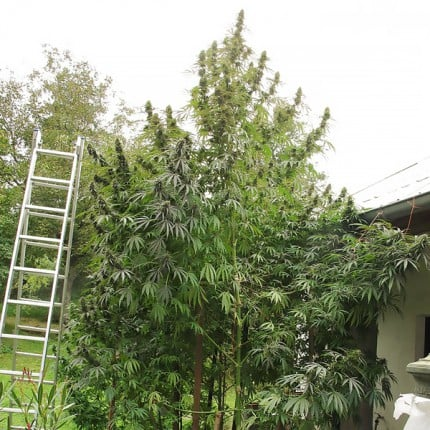
\includegraphics[width=\linewidth]{DUTCH-PASSION_Passion-No1_1}
        \label{fig:cannabis_passion-no1_1}
    \end{subfigure}
    \begin{subfigure}[t]{.48\textwidth}
        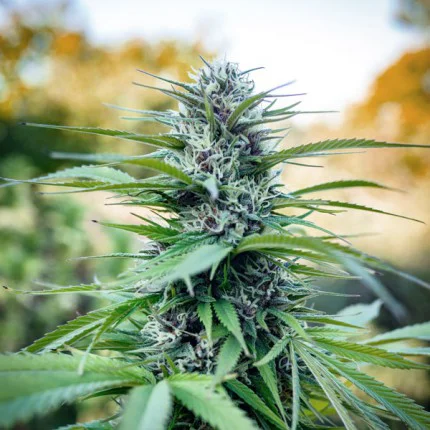
\includegraphics[width=\linewidth]{DUTCH-PASSION_Passion-No1_2}
        \label{fig:cannabis_passion-no1_2}
    \end{subfigure}
    \caption[DUTCH PASSION Passion \#1]{DUTCH PASSION Passion \#1 cultivar. From: \fullcite{noauthor_dutch-passion_passion-no-1_nodate}}
    \label{fig:cannabis_passion-no1}
\end{figure}

\begin{figure}[htbp]
    \begin{subfigure}[t]{.48\textwidth}
        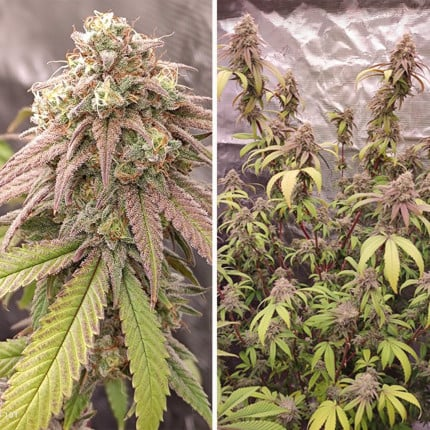
\includegraphics[width=\linewidth]{DUTCH-PASSION_Skywalker-Haze_1}
        \label{fig:cannabis_skywalker-haze_1}
    \end{subfigure}
    \begin{subfigure}[t]{.48\textwidth}
        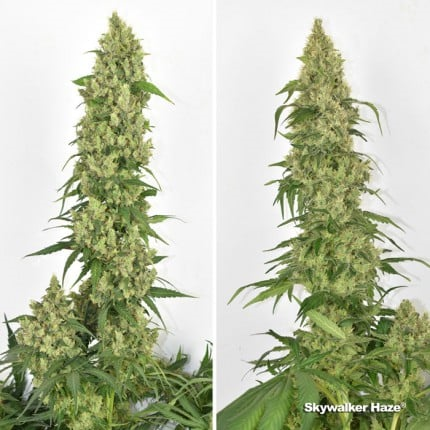
\includegraphics[width=\linewidth]{DUTCH-PASSION_Skywalker-Haze_2}
        \label{fig:cannabis_skywalker-haze_2}
    \end{subfigure}
    \caption[DUTCH PASSION Skywalker Haze]{DUTCH PASSION Skywalker Haze cultivar. From: \fullcite{noauthor_dutch-passion_skywalker-haze_nodate}}
    \label{fig:cannabis_skywalker-haze}
\end{figure}

\begin{figure}[htbp]
    \begin{subfigure}[t]{.48\textwidth}
        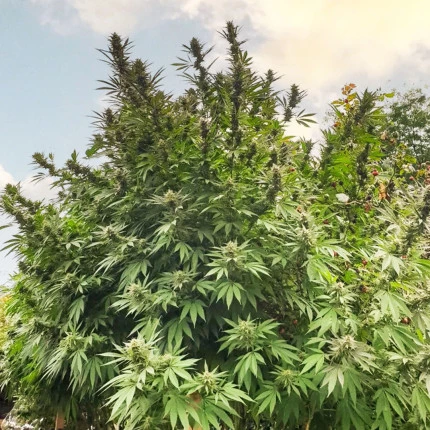
\includegraphics[width=\linewidth]{DUTCH-PASSION_Frisian-Dew_1}
        \label{fig:cannabis_frisian-dew_1}
    \end{subfigure}
    \begin{subfigure}[t]{.48\textwidth}
        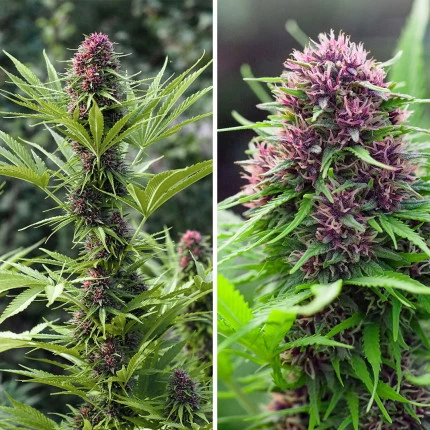
\includegraphics[width=\linewidth]{DUTCH-PASSION_Frisian-Dew_2}
        \label{fig:cannabis_frisian-dew_2}
    \end{subfigure}
    \caption[DUTCH PASSION Frisian Dew]{DUTCH PASSION Frisian Dew cultivar. From: \fullcite{noauthor_dutch-passion_frisian-dew_nodate}}
    \label{fig:cannabis_frisian-dew}
\end{figure}

\begin{figure}[htbp]
    \begin{subfigure}[t]{.48\textwidth}
        \includegraphics[width=\linewidth]{Chiliwelten_3L-Stofftopf-Reißverschluss}
        \caption{\qty[mode=text]{3}{\L} planting container. From: \fullcite{noauthor_chiliwelten_3l_nodate}}
        \label{fig:planting-container-3L}
    \end{subfigure}
    \begin{subfigure}[t]{.48\textwidth}
        \includegraphics[width=\linewidth]{Chiliwelten_15L-Stofftopf-Reißverschluss}
        \caption{\qty[mode=text]{15}{\L} planting container. From: \fullcite{noauthor_chiliwelten_15l_nodate}}
        \label{fig:planting-container-15L}
    \end{subfigure}
    \caption[Planting containers used in this experiment]{The \qty[mode=text]{3}{\L} and \qty[mode=text]{15}{\L} fabric planting containers from Chiliwelten with zipper used in this experiment}
    \label{fig:planting-containers}
\end{figure}

\begin{figure}[htbp]
    \begin{subfigure}[t]{.48\textwidth}
        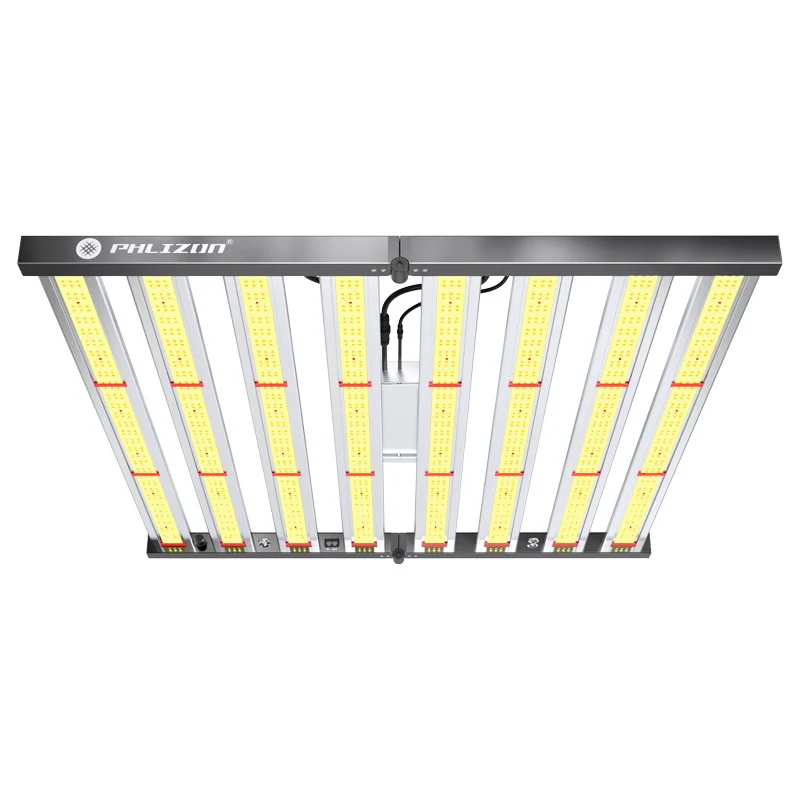
\includegraphics[width=\linewidth]{PHLIZON_PH-FD8-E}
        \label{fig:led_grow_light_img}
    \end{subfigure}
    \begin{subfigure}[t]{.48\textwidth}
        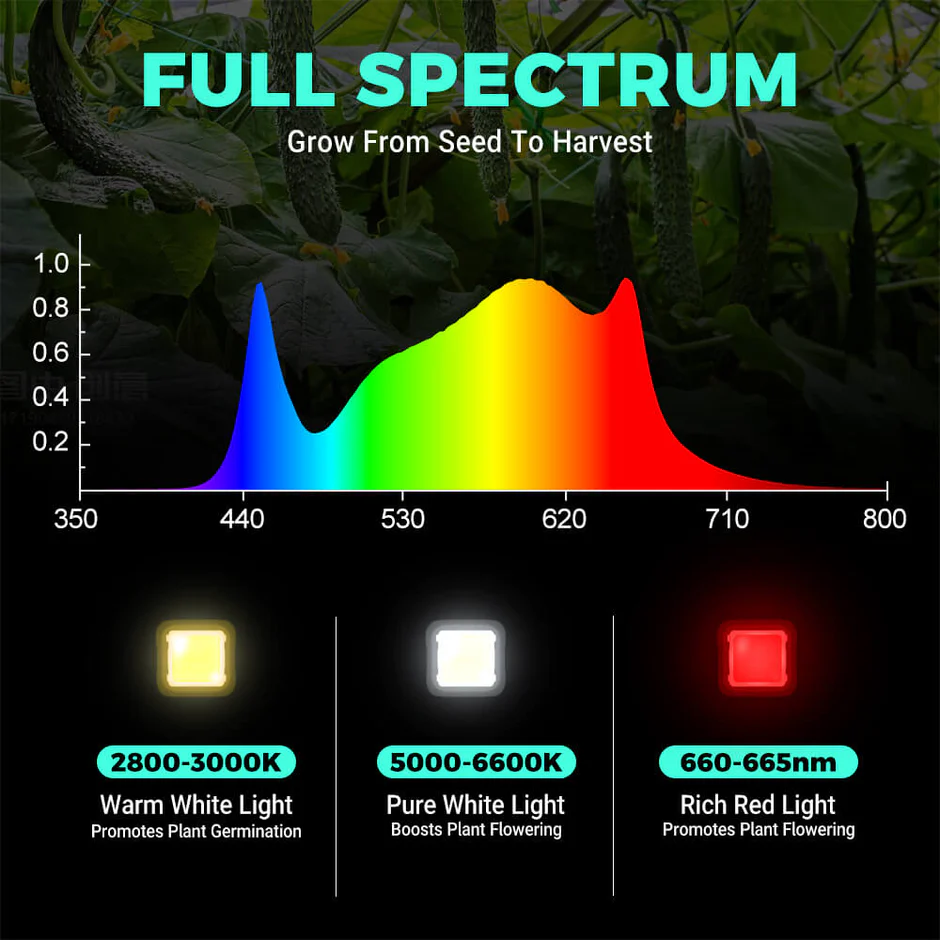
\includegraphics[width=\linewidth]{PHLIZON_PH-FD8-E_light-spectrum}
        \label{fig:led_grow_light_spectrum}
    \end{subfigure}
    \caption[LED grow light used in this experiment]{LED grow light used in this experiment. From \fullcite{noauthor_phlizon_fd6000-640w-upgraded_nodate}}
    \label{fig:led_grow_light}
\end{figure}

\begin{figure}[htbp]
    \begin{subfigure}[t]{.48\textwidth}
        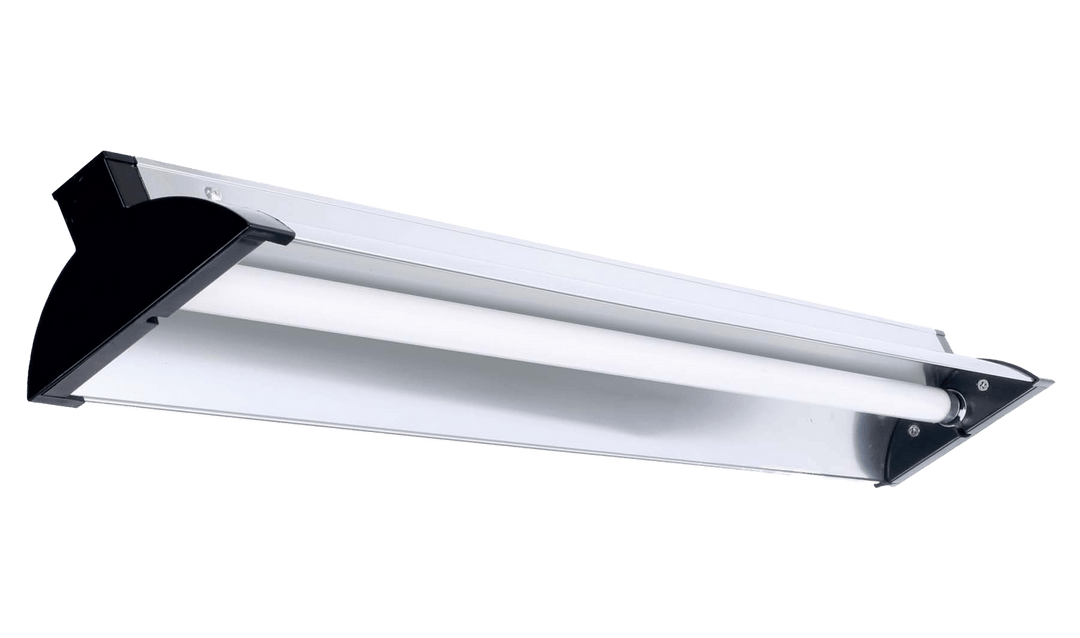
\includegraphics[width=\linewidth]{LuxElite_PlantUV}
        \label{fig:uv_grow_light_img}
    \end{subfigure}
    \begin{subfigure}[t]{.48\textwidth}
        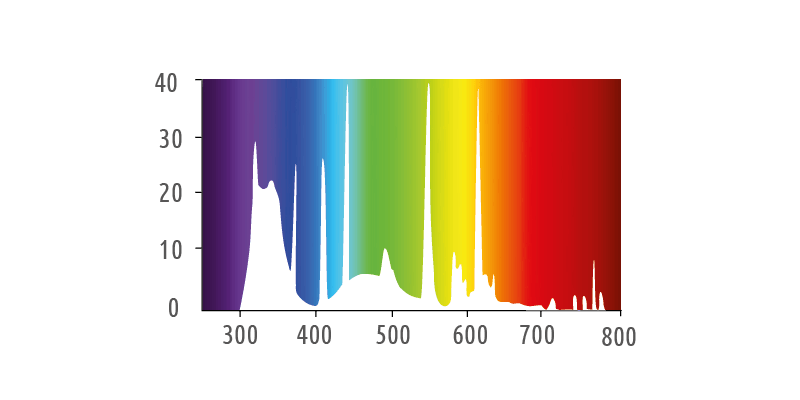
\includegraphics[width=\linewidth]{LuxElite_PlantUV_light-spectrum}
        \label{fig:uv_grow_light_spectrum}
    \end{subfigure}
    \caption[UV grow light used in this experiment]{UV grow light used in this experiment. From \fullcite{noauthor_luxelite_plantuv_nodate}}
    \label{fig:uv_grow_light}
\end{figure}

\subsection{Experimental procedure}

On May 2, ten seeds of DUTCH PASSION Passion \#1 (feminized) and two seeds of DUTCH PASSION Skywalker Haze (feminized) were planted in \qty[mode=text]{3}{\L} fabric planting containers filled with lightly fertilized organic coconut potting soil with added mycorrhizae. The seeds were germinated and initially grown under full-spectrum LED lights (PHLIZON FD6000 PLUS 640W). The plants were divided into two groups, with one group receiving additional light from four LuxElite PlantUV grow lights.

On May 13, these plants were transplanted into \qty[mode=text]{15}{\L} fabric planting containers with fertilized organic coconut potting soil. Additionally, ten seeds of DUTCH PASSION Frisian Dew (regular) were planted in \qty[mode=text]{3}{\L} fabric planting containers under the same conditions. Again, the plants were divided into two groups, with half of the plants receiving supplementary UV light.

On June 16, after \num[mode=text]{45} days of growth for the first set of plants and \num[mode=text]{34} days for the second set, the plants were assessed for the following growth parameters:
\begin{itemize}
    \item Plant height\index{growth parameter!plant height}: Measured from the base of the stem to the highest point using a ruler.
    \item Stem diameter\index{growth parameter!stem diameter}: Measured \qty[mode=text]{2}{\cm} above the soil line using a caliper.
    \item Number of internodes\index{growth parameter!number of internodes}: Counted from the base to the top of the plant.
\end{itemize}

Additionally, light conditions were measured using a THORLABS CCS200/M light spectrometer\index{light spectrometer!THORLABS CCS200/M}.

\subsection{Growing conditions}

The temperature\index{growing condition!temperature} was maintained at about \qty[mode=text]{21}{\degreeCelsius}. The height of the grow lights\index{grow light} was adjusted to maintain a distance of approximately \qty[mode=text]{20}{\cm} from the tip of the tallest plant. The LED grow lights\index{grow light!LED} were set to \qty[mode=text]{100}{\percent} dimmable intensity. All lights were on daily from 5:35 a.m. to 9:35 p.m. (\qty[mode=text]{16}{hr} daily). On June 16, the local sunrise was at 5:18 a.m. and the sunset was at 9:52 p.m.

    \newpage
    \section{Results}

Table \ref{tab:measured_growth_parameters} shows the measured growth parameters: plant height\index{growth parameter!plant height}, stem circumference\index{growth parameter!stem circumference}, and number of internodes\index{growth parameter!number of internodes} at the end of the experiment after \num[mode=text]{46} days for both the UV and the control groups. Note that plant number \num[mode=text]{4} (control) died.

Figures \ref{fig:plants_uv_2024-05-13} and \ref{fig:plants_ctrl_2024-05-13} show the plants treated with UV light and the plants of the control group, respectively, on May 13 when the plants were transplanted into \qty[mode=text]{15}{\L} containers. Figures \ref{fig:plants_uv_2024-06-17} and \ref{fig:plants_ctrl_2024-06-17} show the plants of the UV and control groups, respectively, on June 17, including their experimental setups. Figure \ref{fig:plant_all_2024-06-17} shows all plants together on June 17.

\begin{table}[htbp]
    \caption[Measured growth parameters of the cannabis plants]{Measured growth parameters of the cannabis plants on June 17, \num[mode=text]{46} days after planting the seeds.}
    \label{tab:measured_growth_parameters}
    \begin{tabularx}{\linewidth}{llcccc}
        \toprule
        \textbf{Group} & \textbf{Cultivar} & \textbf{Plant \#} & \textbf{Height (\unit[mode=text]{\cm})} & \textbf{Stem cir. (\unit[mode=text]{\cm})} & \textbf{\#{}Internodes} \\
        \midrule
        \multirow{6}{*}{UV} & Skywalker Haze & 1 & 49 & 4.3 & 11 \\
        & \multirow[t]{5}{*}{Frisian Dew} & 3 & 59 & 5.5 & 12 \\
        & & 5 & 56 & 5.5 & 12 \\
        & & 7 & 54 & 5.1 & 11 \\
        & & 9 & 56 & 5.5 & 12 \\
        & & 11 & 52 & 4.7 & 12 \\
        \midrule
        \multirow{6}{*}{Control} & Skywalker Haze & 2 & 49 & 5.0 & 12 \\
        & \multirow[t]{5}{*}{Frisian Dew} & 4 & - & - & - \\
        & & 6 & 49 & 6.0 & 13 \\
        & & 8 & 60 & 5.5 & 12 \\
        & & 10 & 69 & 5.0 & 12 \\
        & & 12 & 52 & 5.8 & 12 \\
        \bottomrule
    \end{tabularx}
\end{table}

\subsection{Statistical analysis}

\subsubsection{Initial hypothesis}

The initial hypothesis of this experiment was: "Exposure to UV-A light at controlled low intensities enhances the germination rate and seedling development of Cannabis seeds by inducing protective and growth-promoting biochemical responses."

\subsubsection{Analysis procedure}

For the statistical analysis, we focused only on the Frisian Dew cultivar since there is only one Skywalker Haze plant in each group, which is insufficient for deriving statistical conclusions. The following statistical analyses were conducted:
\begin{enumerate}
    \item \emph{Descriptive statistics:} Calculation of mean and standard deviation for each growth parameter (plant height, stem circumference, and number of internodes) in both groups.
    \item \emph{Welch's t-test\index{statistics!Welch's t-test}:} Comparison of means between the UV and control groups for each growth parameter to determine if there were significant differences.
\end{enumerate}

\subsubsection{Descriptive statistics}

Table \ref{tab:descriptive_statistics} provides the mean\index{statistics!mean} and standard deviation\index{statistics!standard deviation} for the growth parameters of the Frisian Dew cultivar in both the UV and control groups. These statistics are essential for understanding the variability and central tendency of the measured growth parameters within each group.

\begin{table}[htbp]
    \caption[Mean and standard deviation of growth parameters]{Mean and standard deviation of growth parameters for Frisian Dew cultivar}
    \label{tab:descriptive_statistics}
    \begin{tabularx}{\linewidth}{l|XX|XX|XX}
        \toprule
        \textbf{Group} & \multicolumn{2}{l|}{\textbf{Height (\unit[mode=text]{\cm})}} & \multicolumn{2}{l|}{\textbf{Stem cir. (\unit[mode=text]{\cm})}} & \multicolumn{2}{l}{\textbf{\# Internodes}} \\
        & \textbf{Mean} & \textbf{SD} & \textbf{Mean} & \textbf{SD} & \textbf{Mean} & \textbf{SD} \\
        \midrule
        UV & \num[mode=text]{55} & \num[mode=text]{2.6} & \num[mode=text]{5.3} & \num[mode=text]{0.36} & \num[mode=text]{12} & \num[mode=text]{0.45} \\
        Control & \num[mode=text]{58} & \num[mode=text]{9.0} & \num[mode=text]{5.6} & \num[mode=text]{0.43} & \num[mode=text]{12} & \num[mode=text]{0.50} \\
        \bottomrule
    \end{tabularx}
\end{table}

\subsubsection{T-test analysis}

To compare the growth parameters between the UV and control groups for the Frisian Dew cultivar, an independent samples t-test (Welch's t-test\index{statistics!Welch's t-test}) was conducted. This type of t-test is used to determine if there is a statistically significant difference between the means of two groups. The test assumes that the two groups are independent and that the data are approximately normally distributed, without assuming equal variances between groups.

The results of the t-tests for plant height, stem circumference, and number of internodes are presented in Table \ref{tab:ttest_results}. These results indicate no significant differences between the UV and control groups for any of the measured growth parameters, suggesting that UV light exposure did not significantly influence these parameters under the conditions of this experiment.

Therefore, these findings do not support the initial hypothesis that UV light enhances germination rate and seedling development through protective and growth-promoting biochemical responses.

\begin{table}[htbp]
    \caption{Welch's t-test results for growth parameters}
    \label{tab:ttest_results}
    \begin{tabularx}{\linewidth}{lcc}
        \toprule
        \textbf{Parameter} & \textbf{t-value} & \textbf{p-value} \\
        \midrule
        Plant height & \num[mode=text]{-0.45} & \num[mode=text]{0.68} \\
        Stem cir. & \num[mode=text]{-1.17} & \num[mode=text]{0.29} \\
        \# Internodes & \num[mode=text]{-1.41} & \num[mode=text]{0.21} \\
        \bottomrule
    \end{tabularx}
\end{table}

\begin{figure}[htbp]
    \begin{subfigure}[t]{.19\textwidth}
        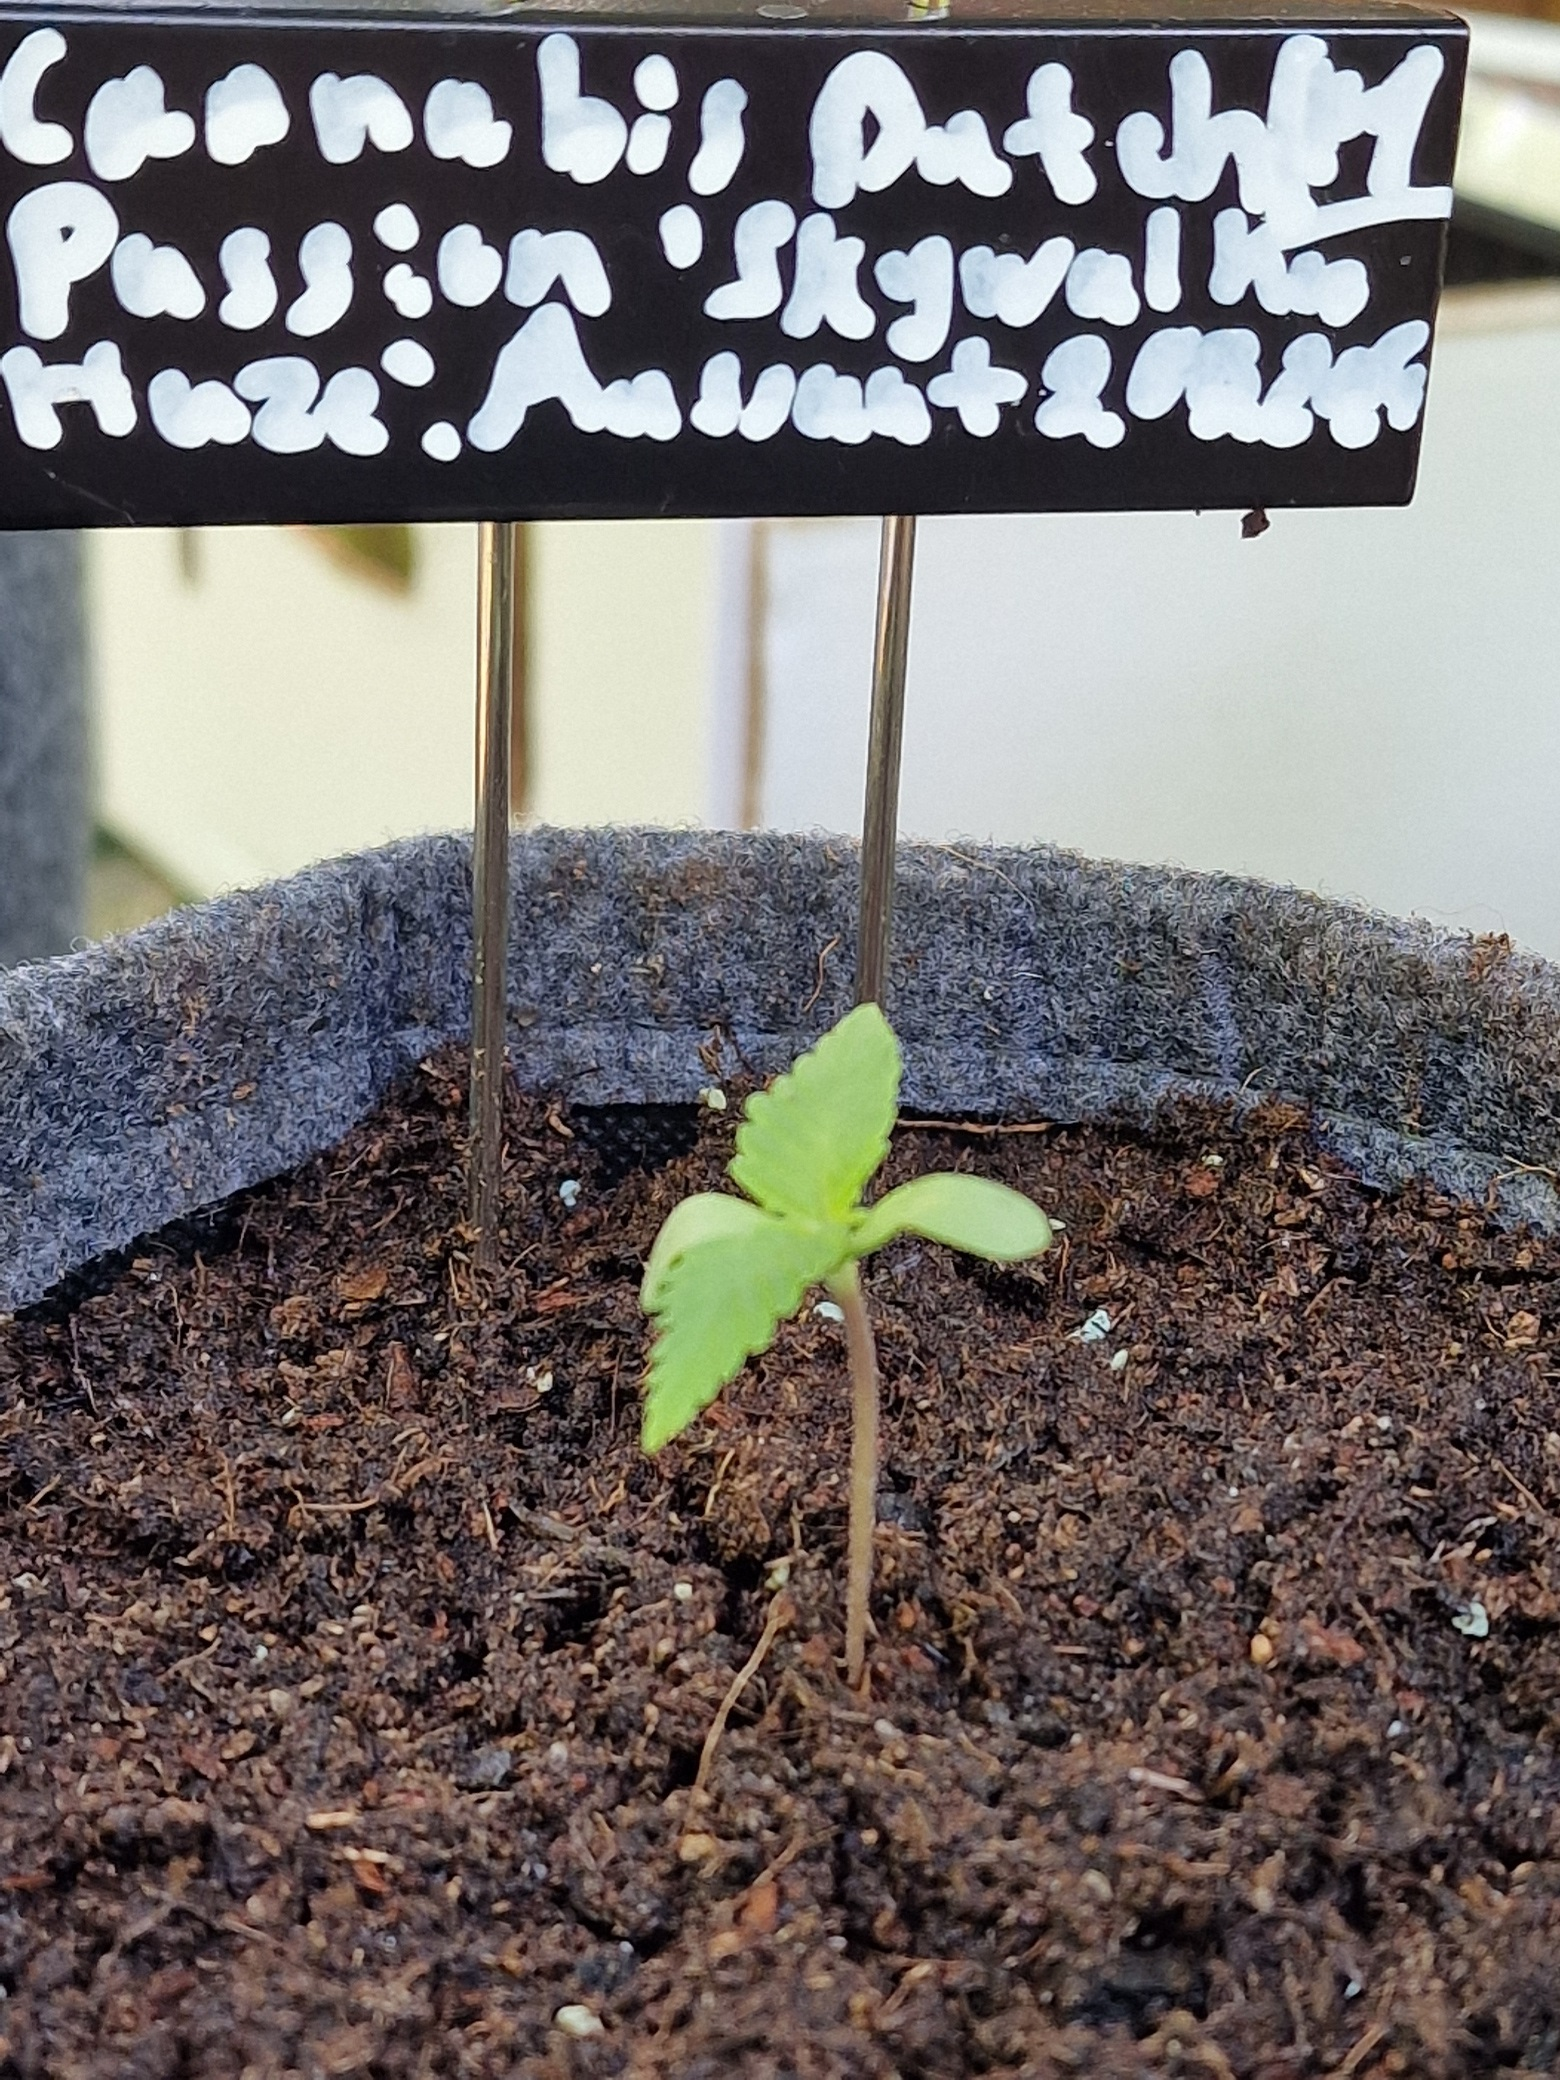
\includegraphics[width=\linewidth]{plant_01_2024-05-13}
        \caption{Plant \# 1}
        \label{fig:plant_01_2024-05-13}
    \end{subfigure}
    \begin{subfigure}[t]{.19\textwidth}
        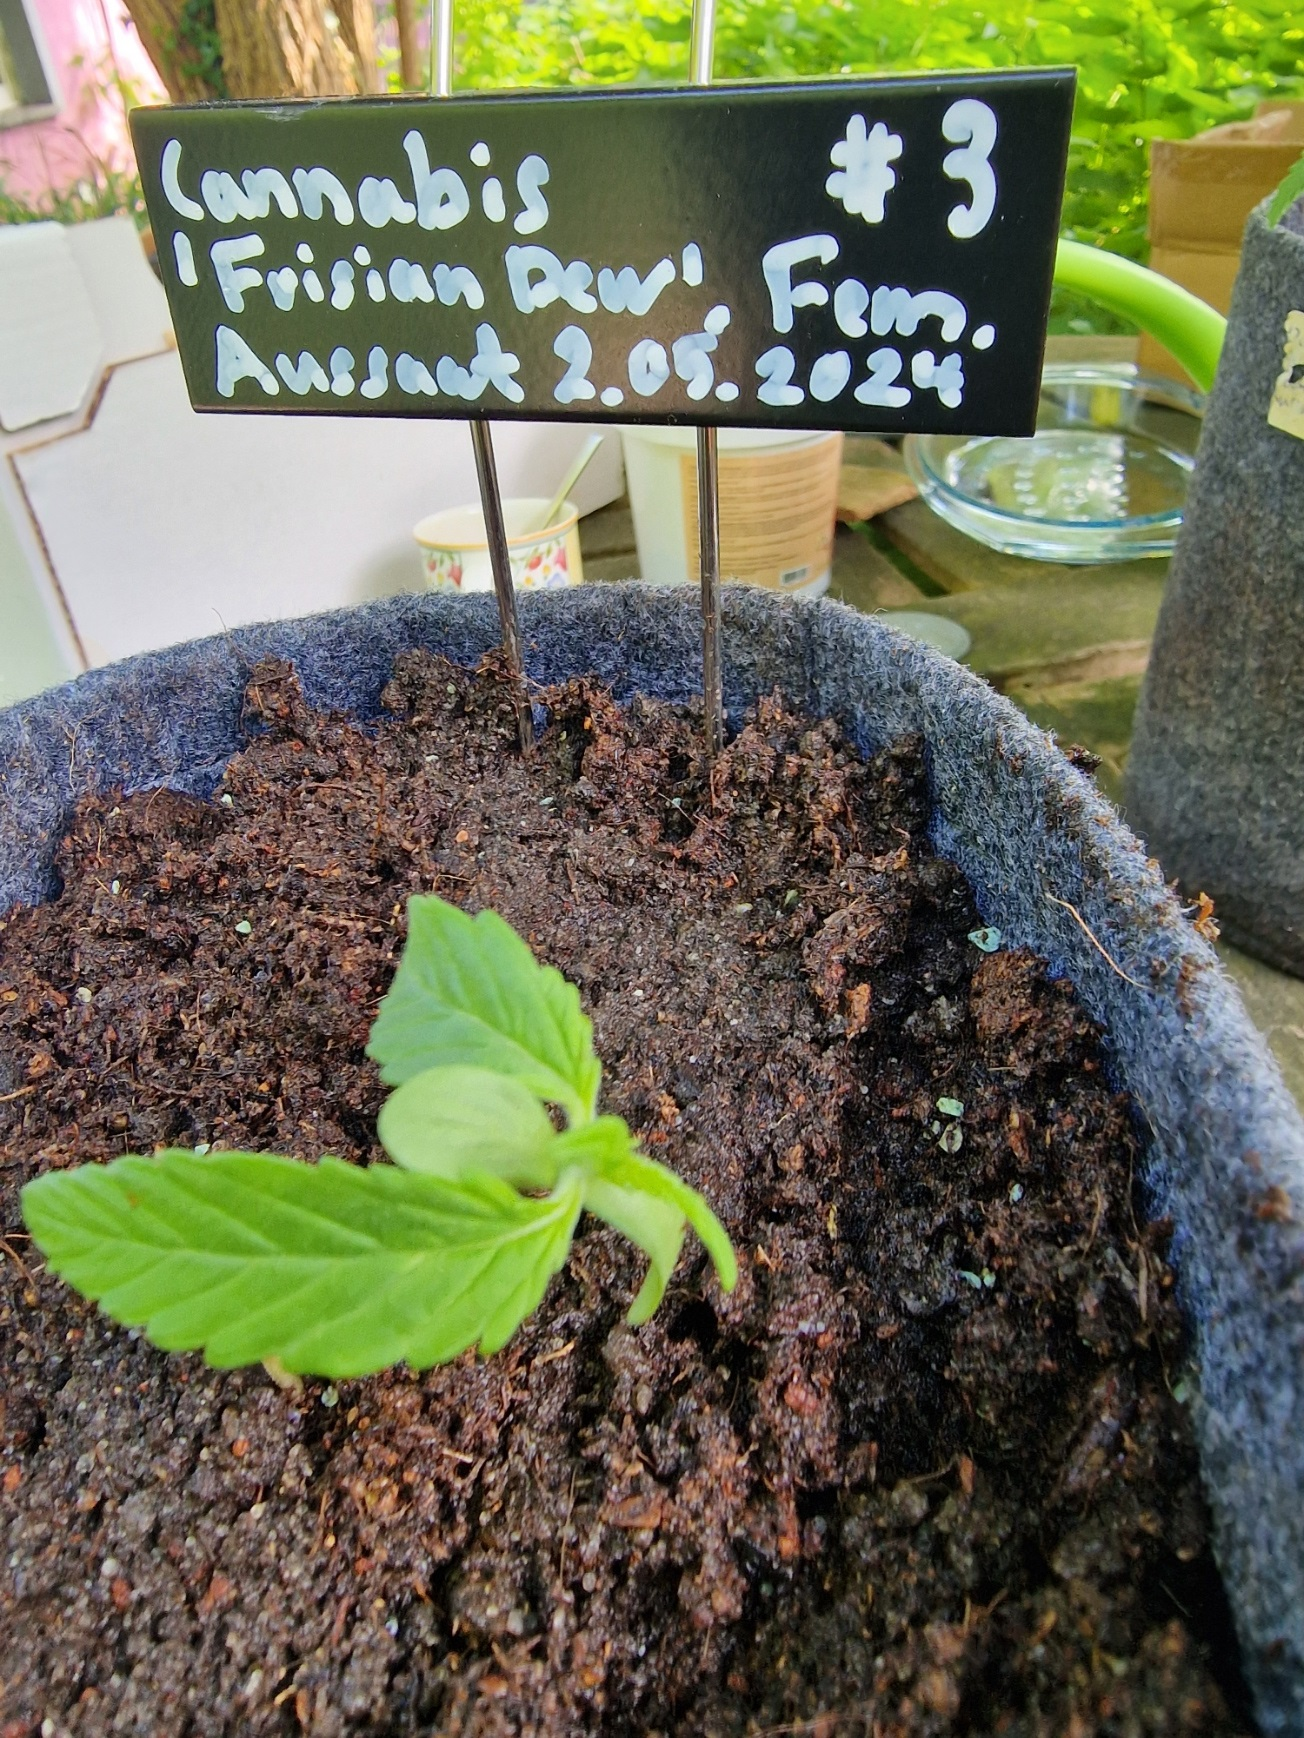
\includegraphics[width=\linewidth]{plant_03_2024-05-13}
        \caption{Plant \# 3}
        \label{fig:plant_03_2024-05-13}
    \end{subfigure}
    \begin{subfigure}[t]{.19\textwidth}
        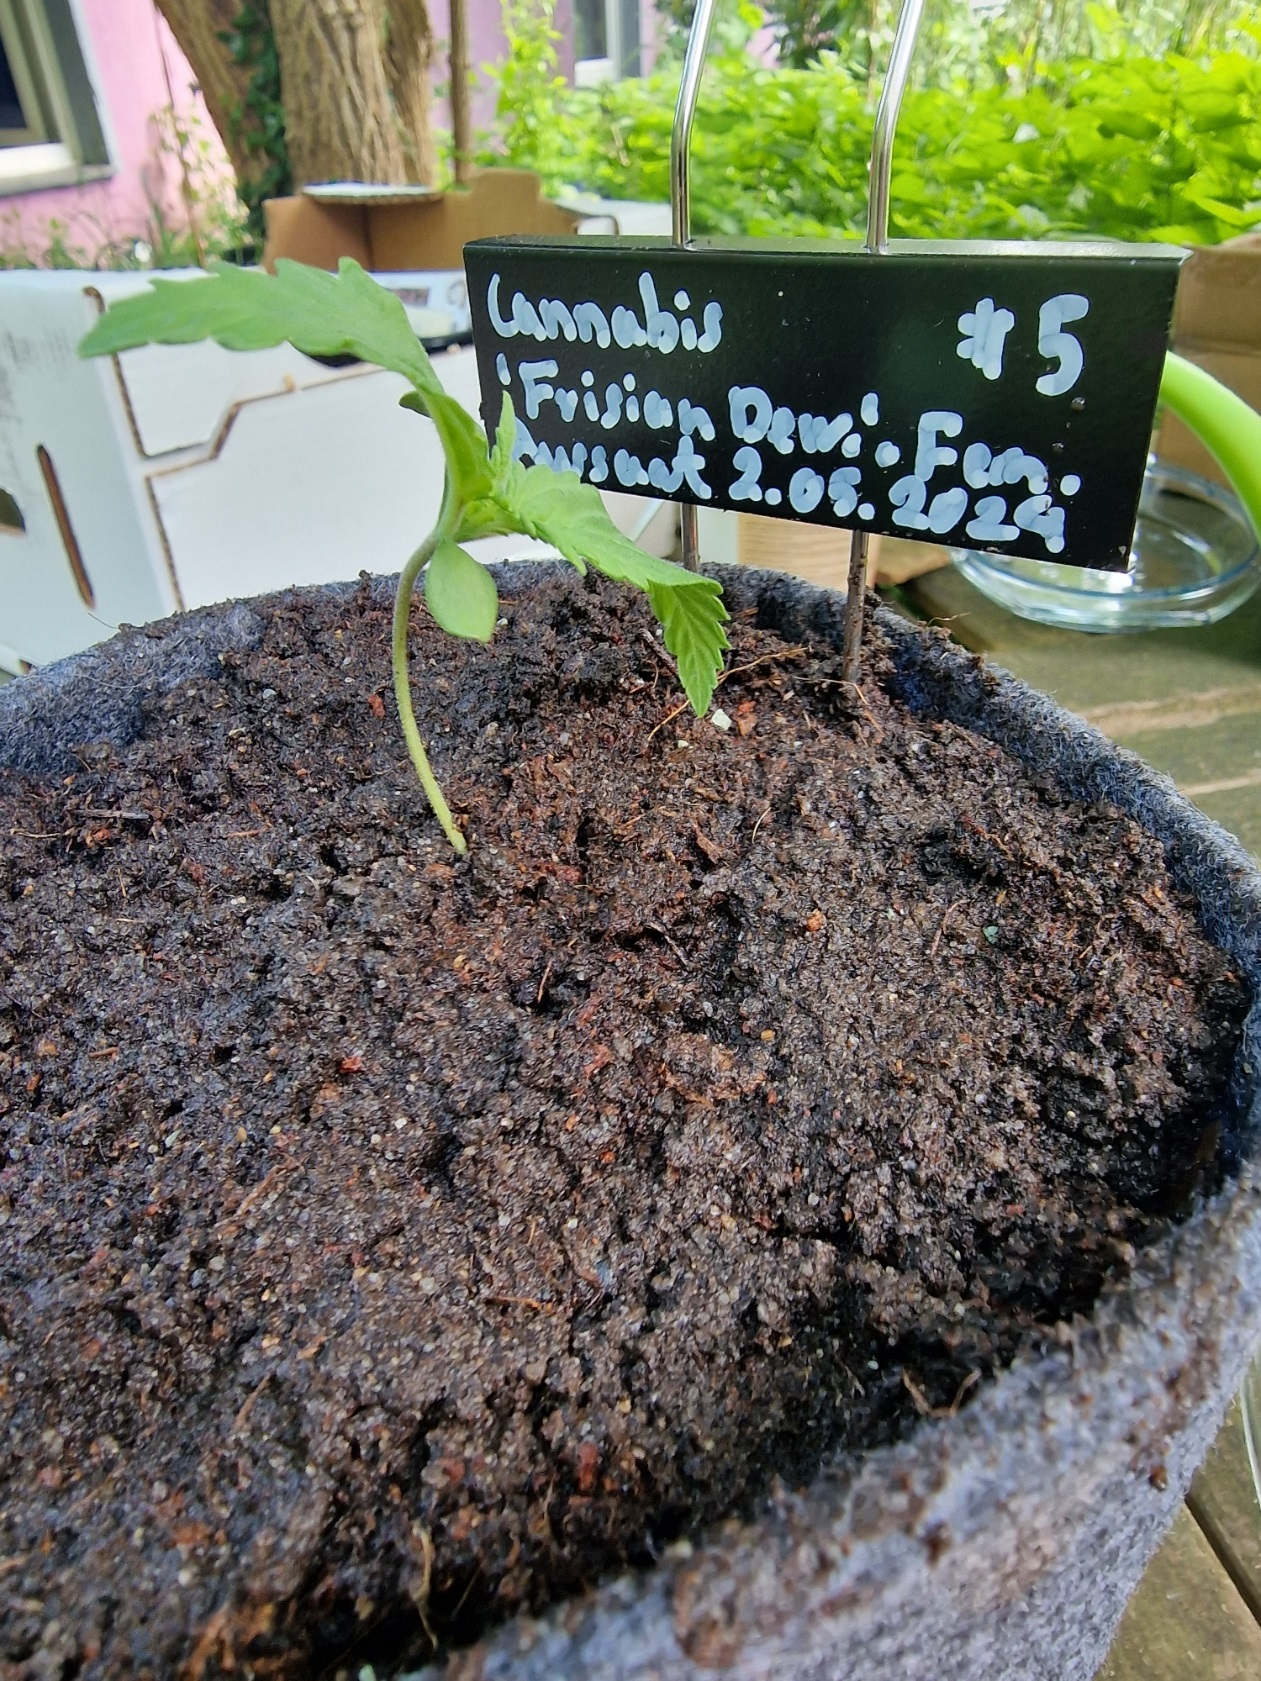
\includegraphics[width=\linewidth]{plant_05_2024-05-13}
        \caption{Plant \# 5}
        \label{fig:plant_05_2024-05-13}
    \end{subfigure}
    \begin{subfigure}[t]{.19\textwidth}
        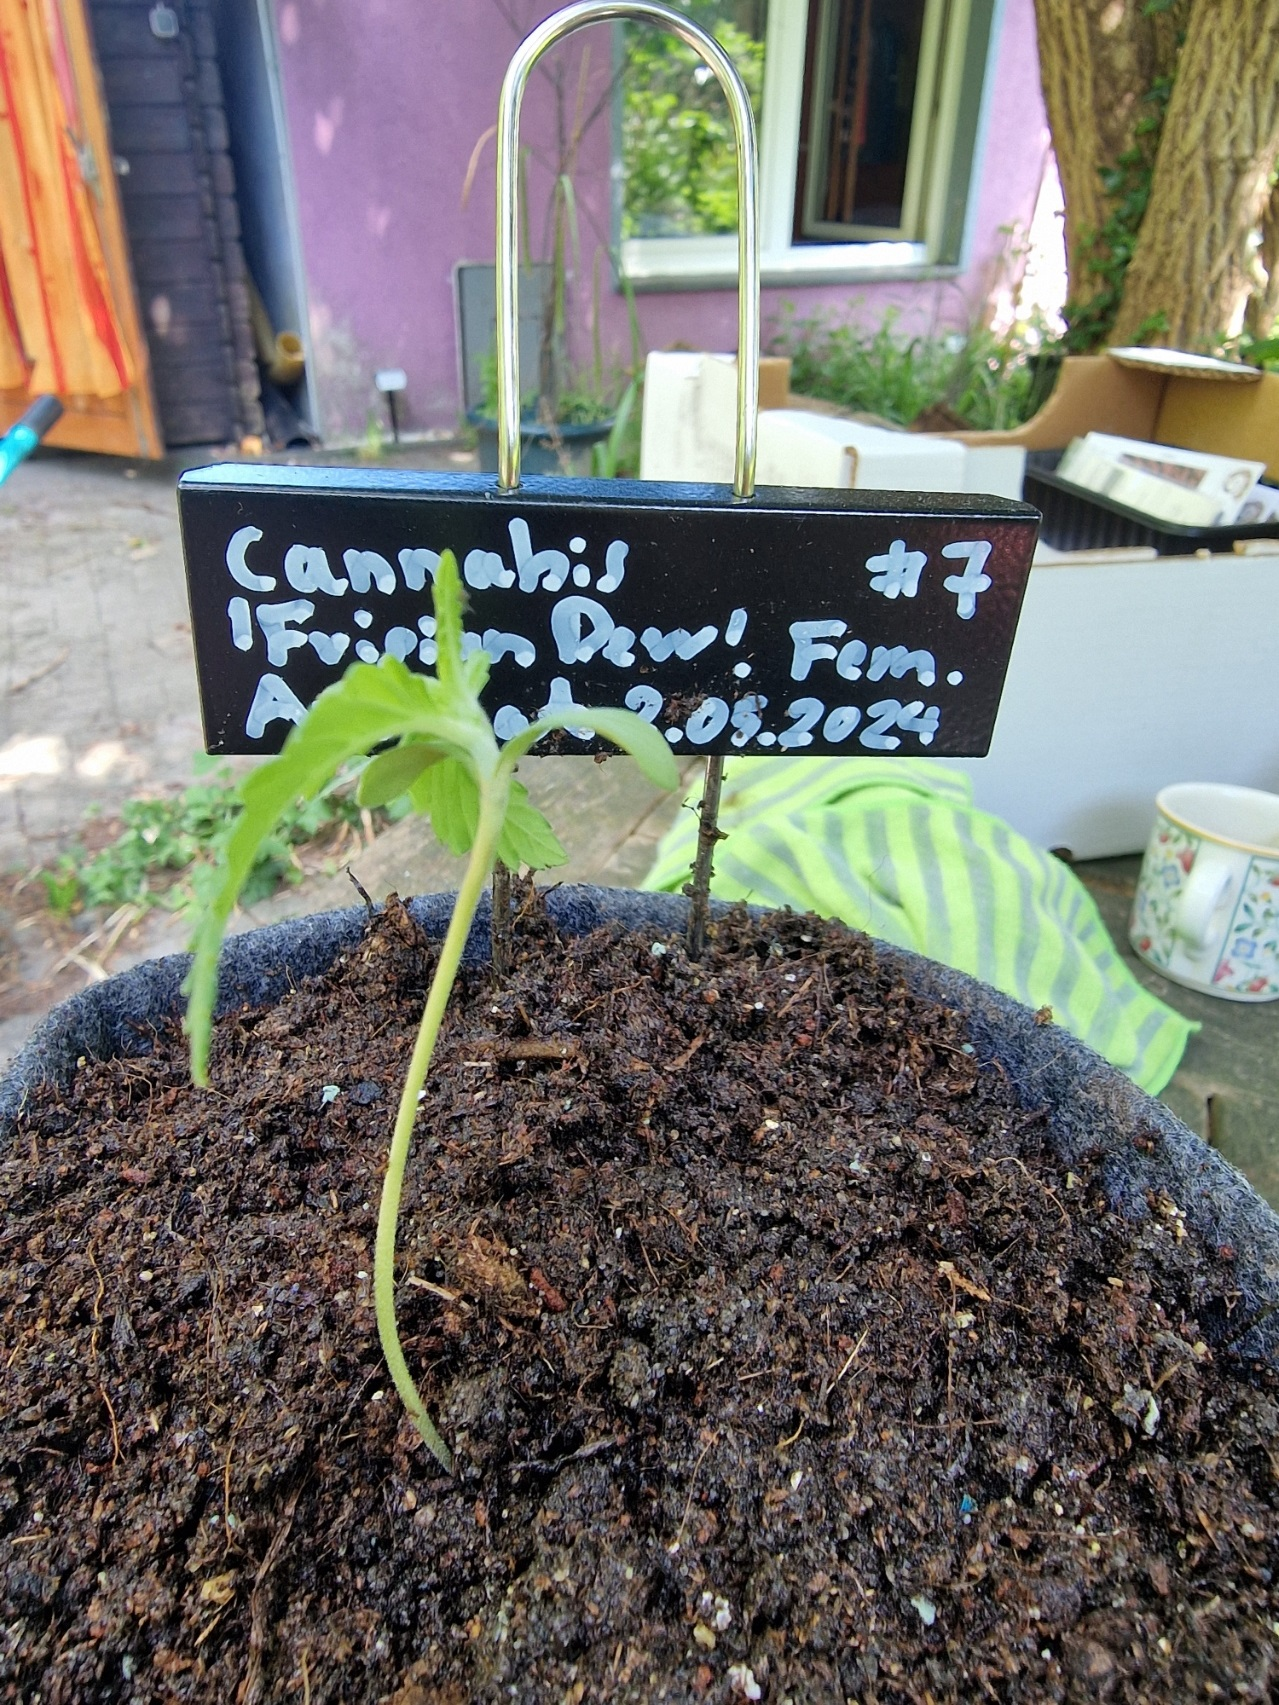
\includegraphics[width=\linewidth]{plant_07_2024-05-13}
        \caption{Plant \# 7}
        \label{fig:plant_07_2024-05-13}
    \end{subfigure}
    \begin{subfigure}[t]{.19\textwidth}
        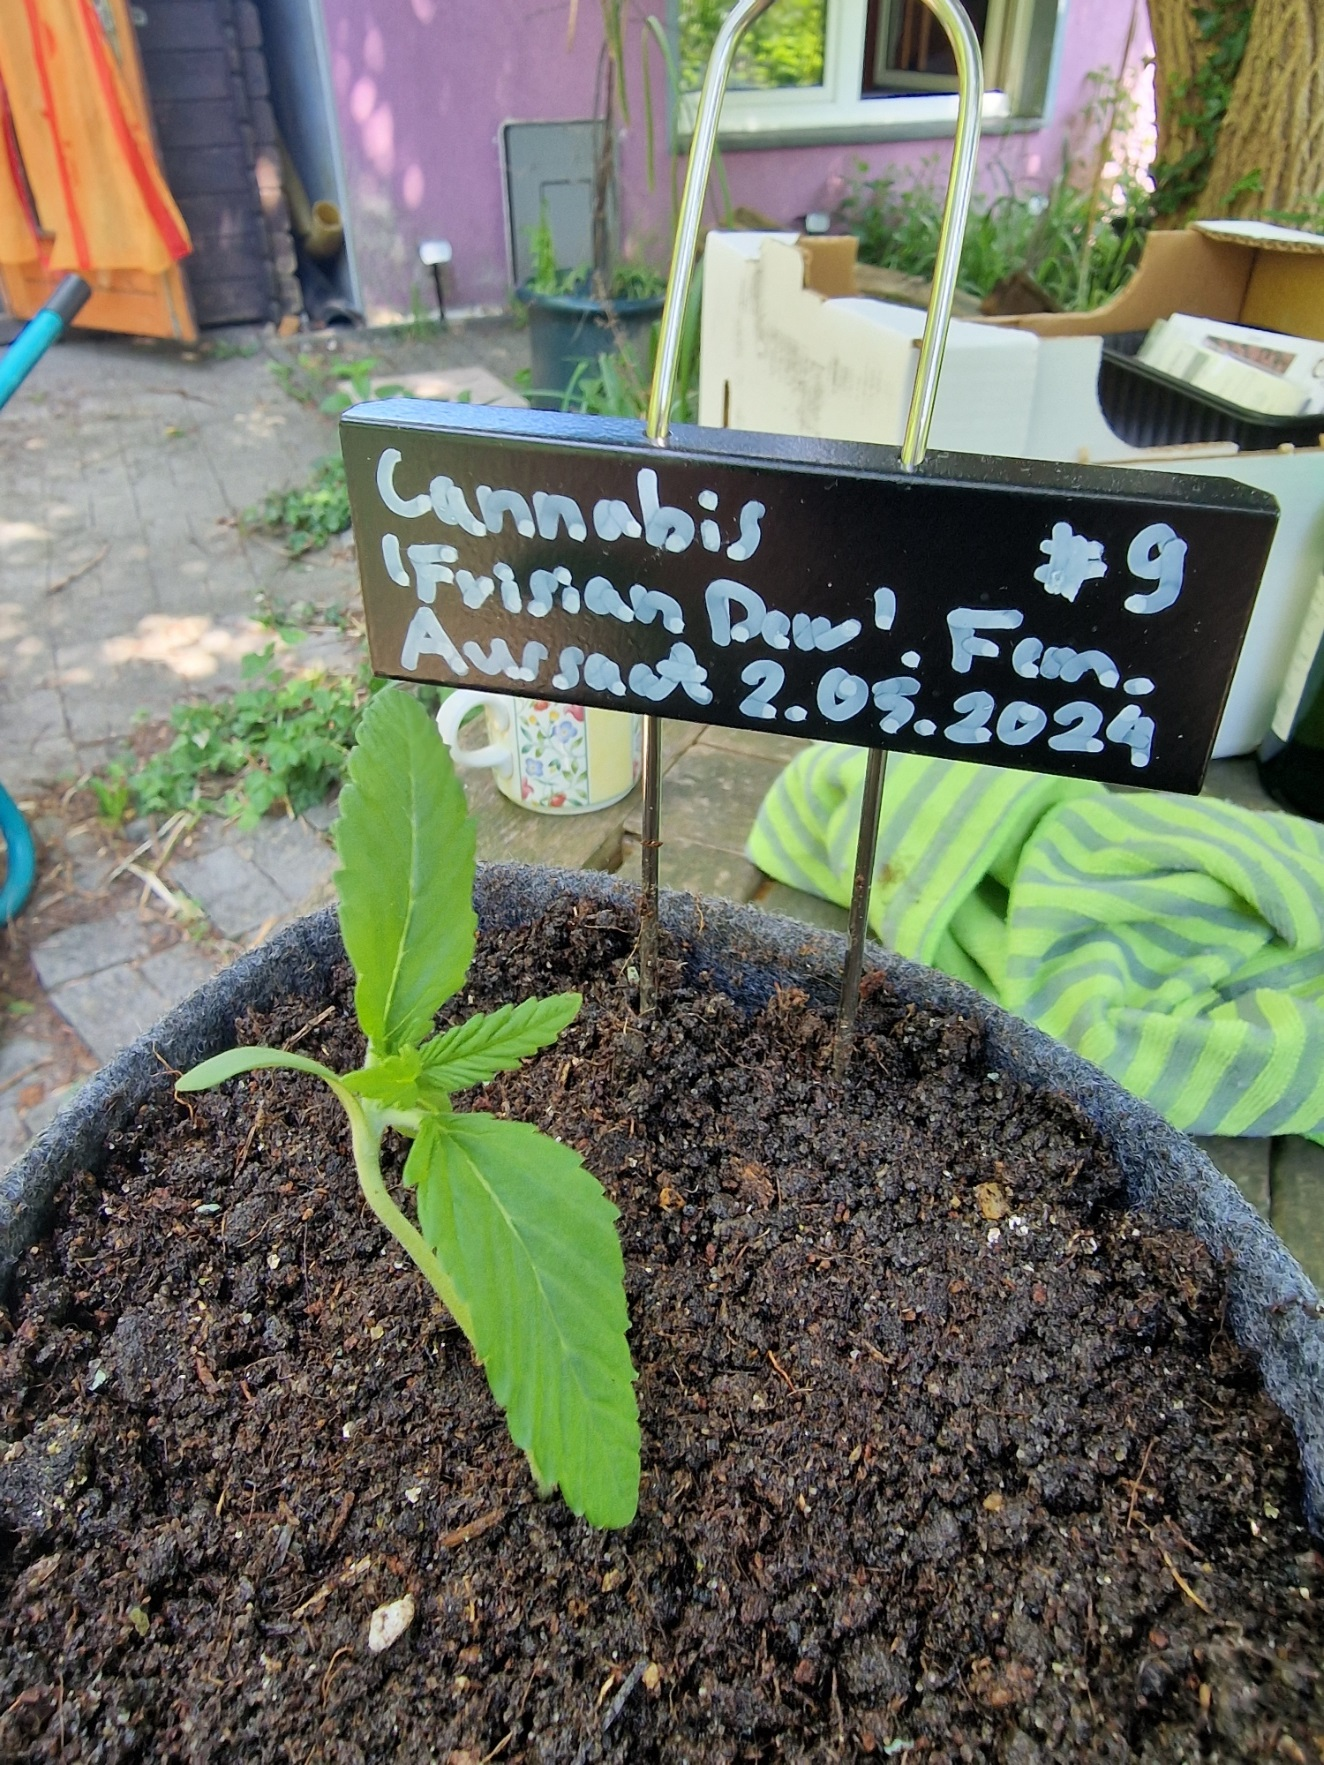
\includegraphics[width=\linewidth]{plant_09_2024-05-13}
        \caption{Plant \# 9}
        \label{fig:plant_09_2024-05-13}
    \end{subfigure}
    \caption[Plants of the UV group on May 13]{The plants treated with UV light on May 13}
    \label{fig:plants_uv_2024-05-13}
\end{figure}

\begin{figure}[htbp]
    \begin{subfigure}[t]{.19\textwidth}
        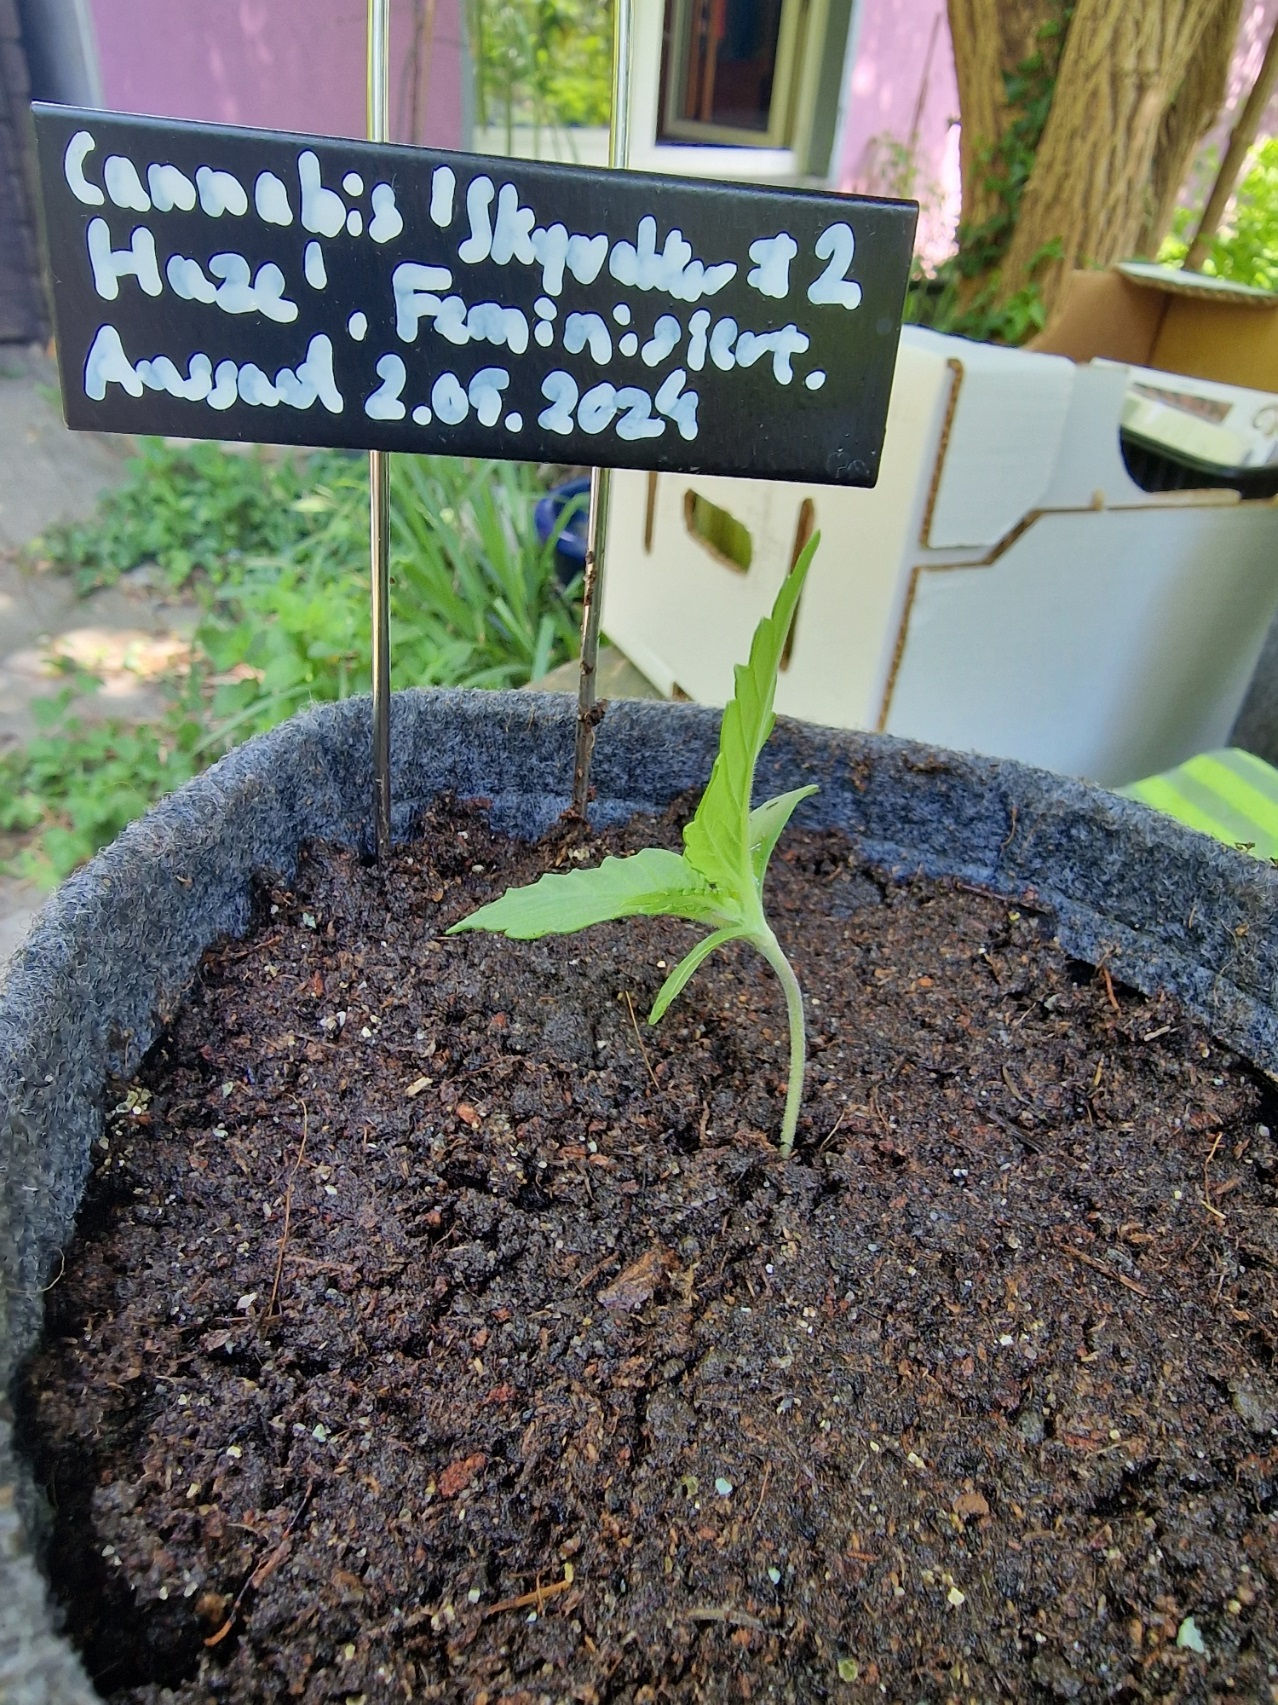
\includegraphics[width=\linewidth]{plant_02_2024-05-13}
        \caption{Plant \# 2}
        \label{fig:plant_02_2024-05-13}
    \end{subfigure}
    \begin{subfigure}[t]{.19\textwidth}
        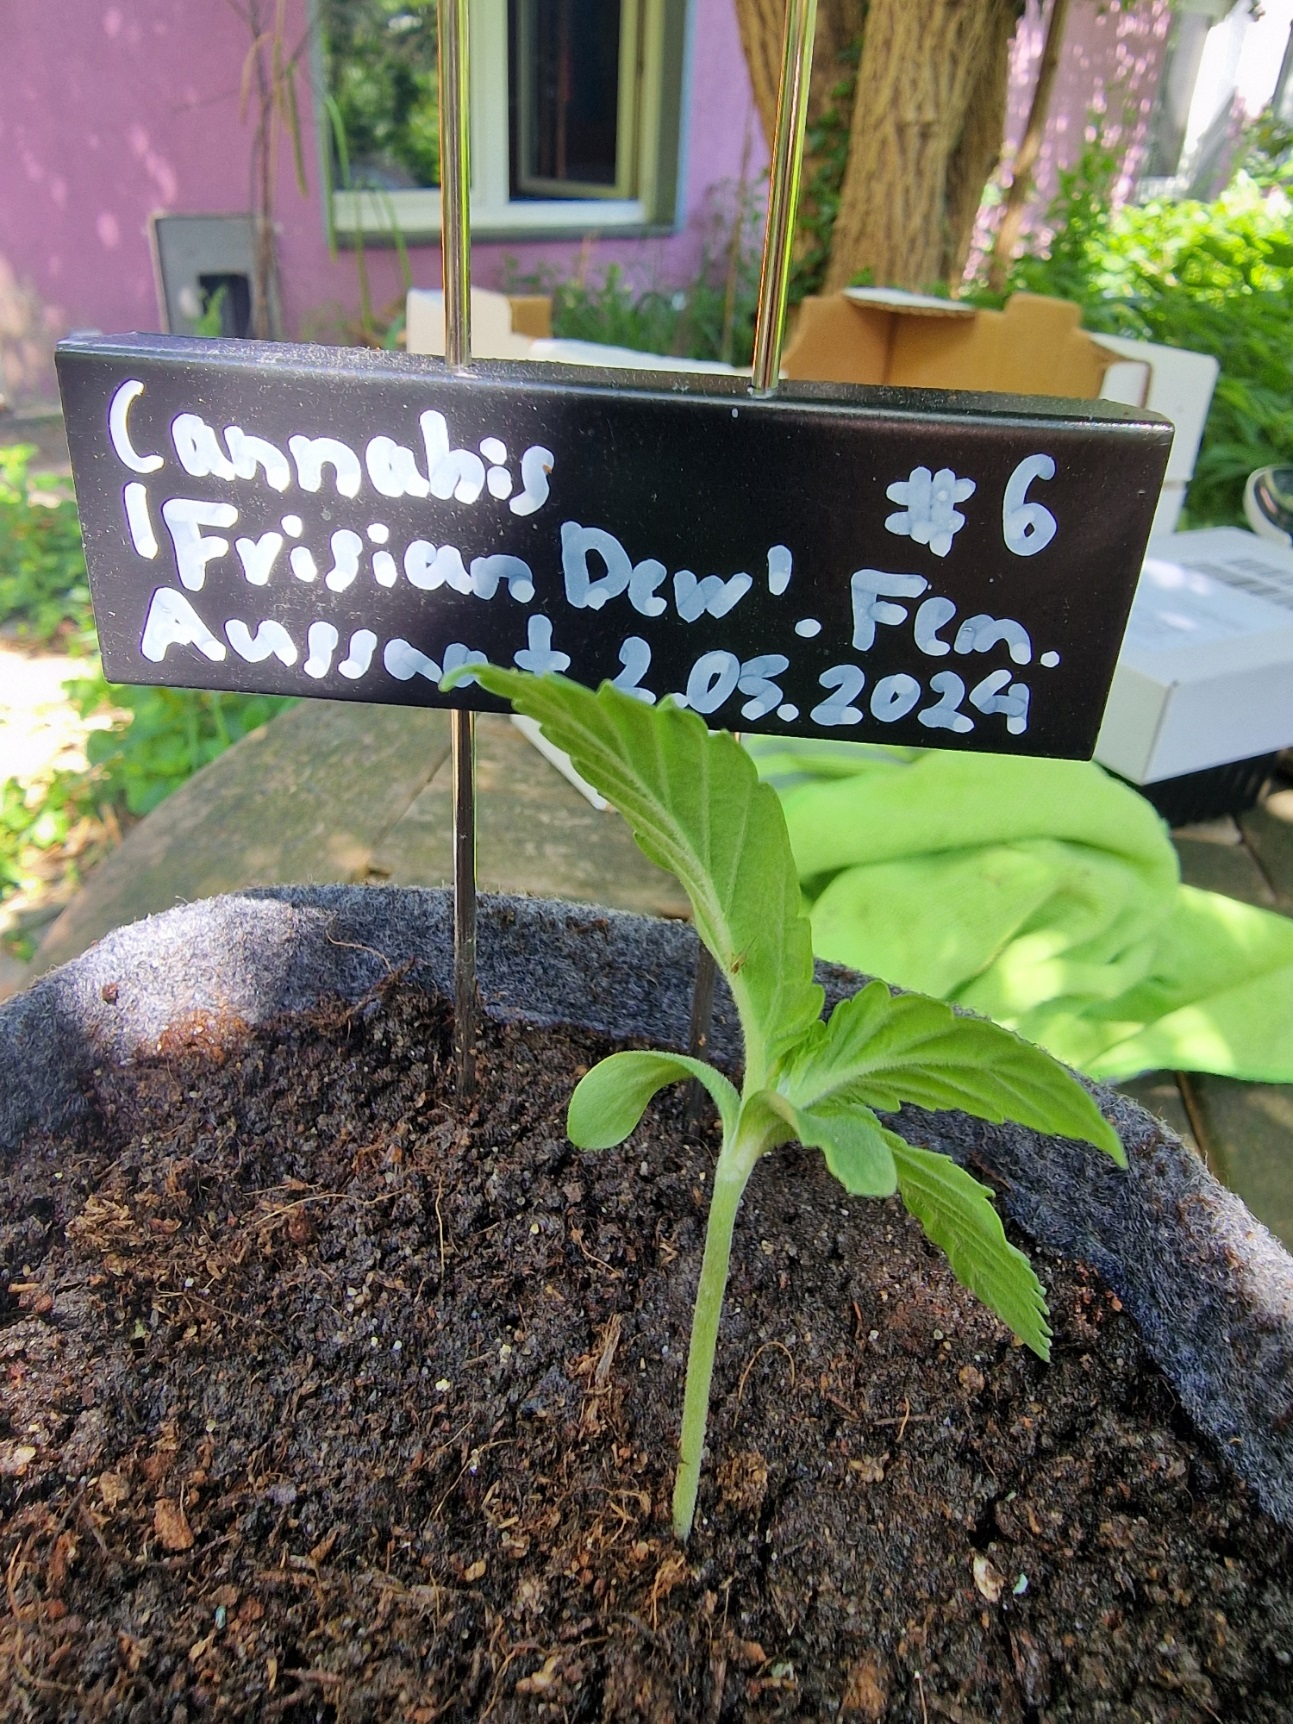
\includegraphics[width=\linewidth]{plant_06_2024-05-13}
        \caption{Plant \# 6}
        \label{fig:plant_06_2024-05-13}
    \end{subfigure}
    \begin{subfigure}[t]{.19\textwidth}
        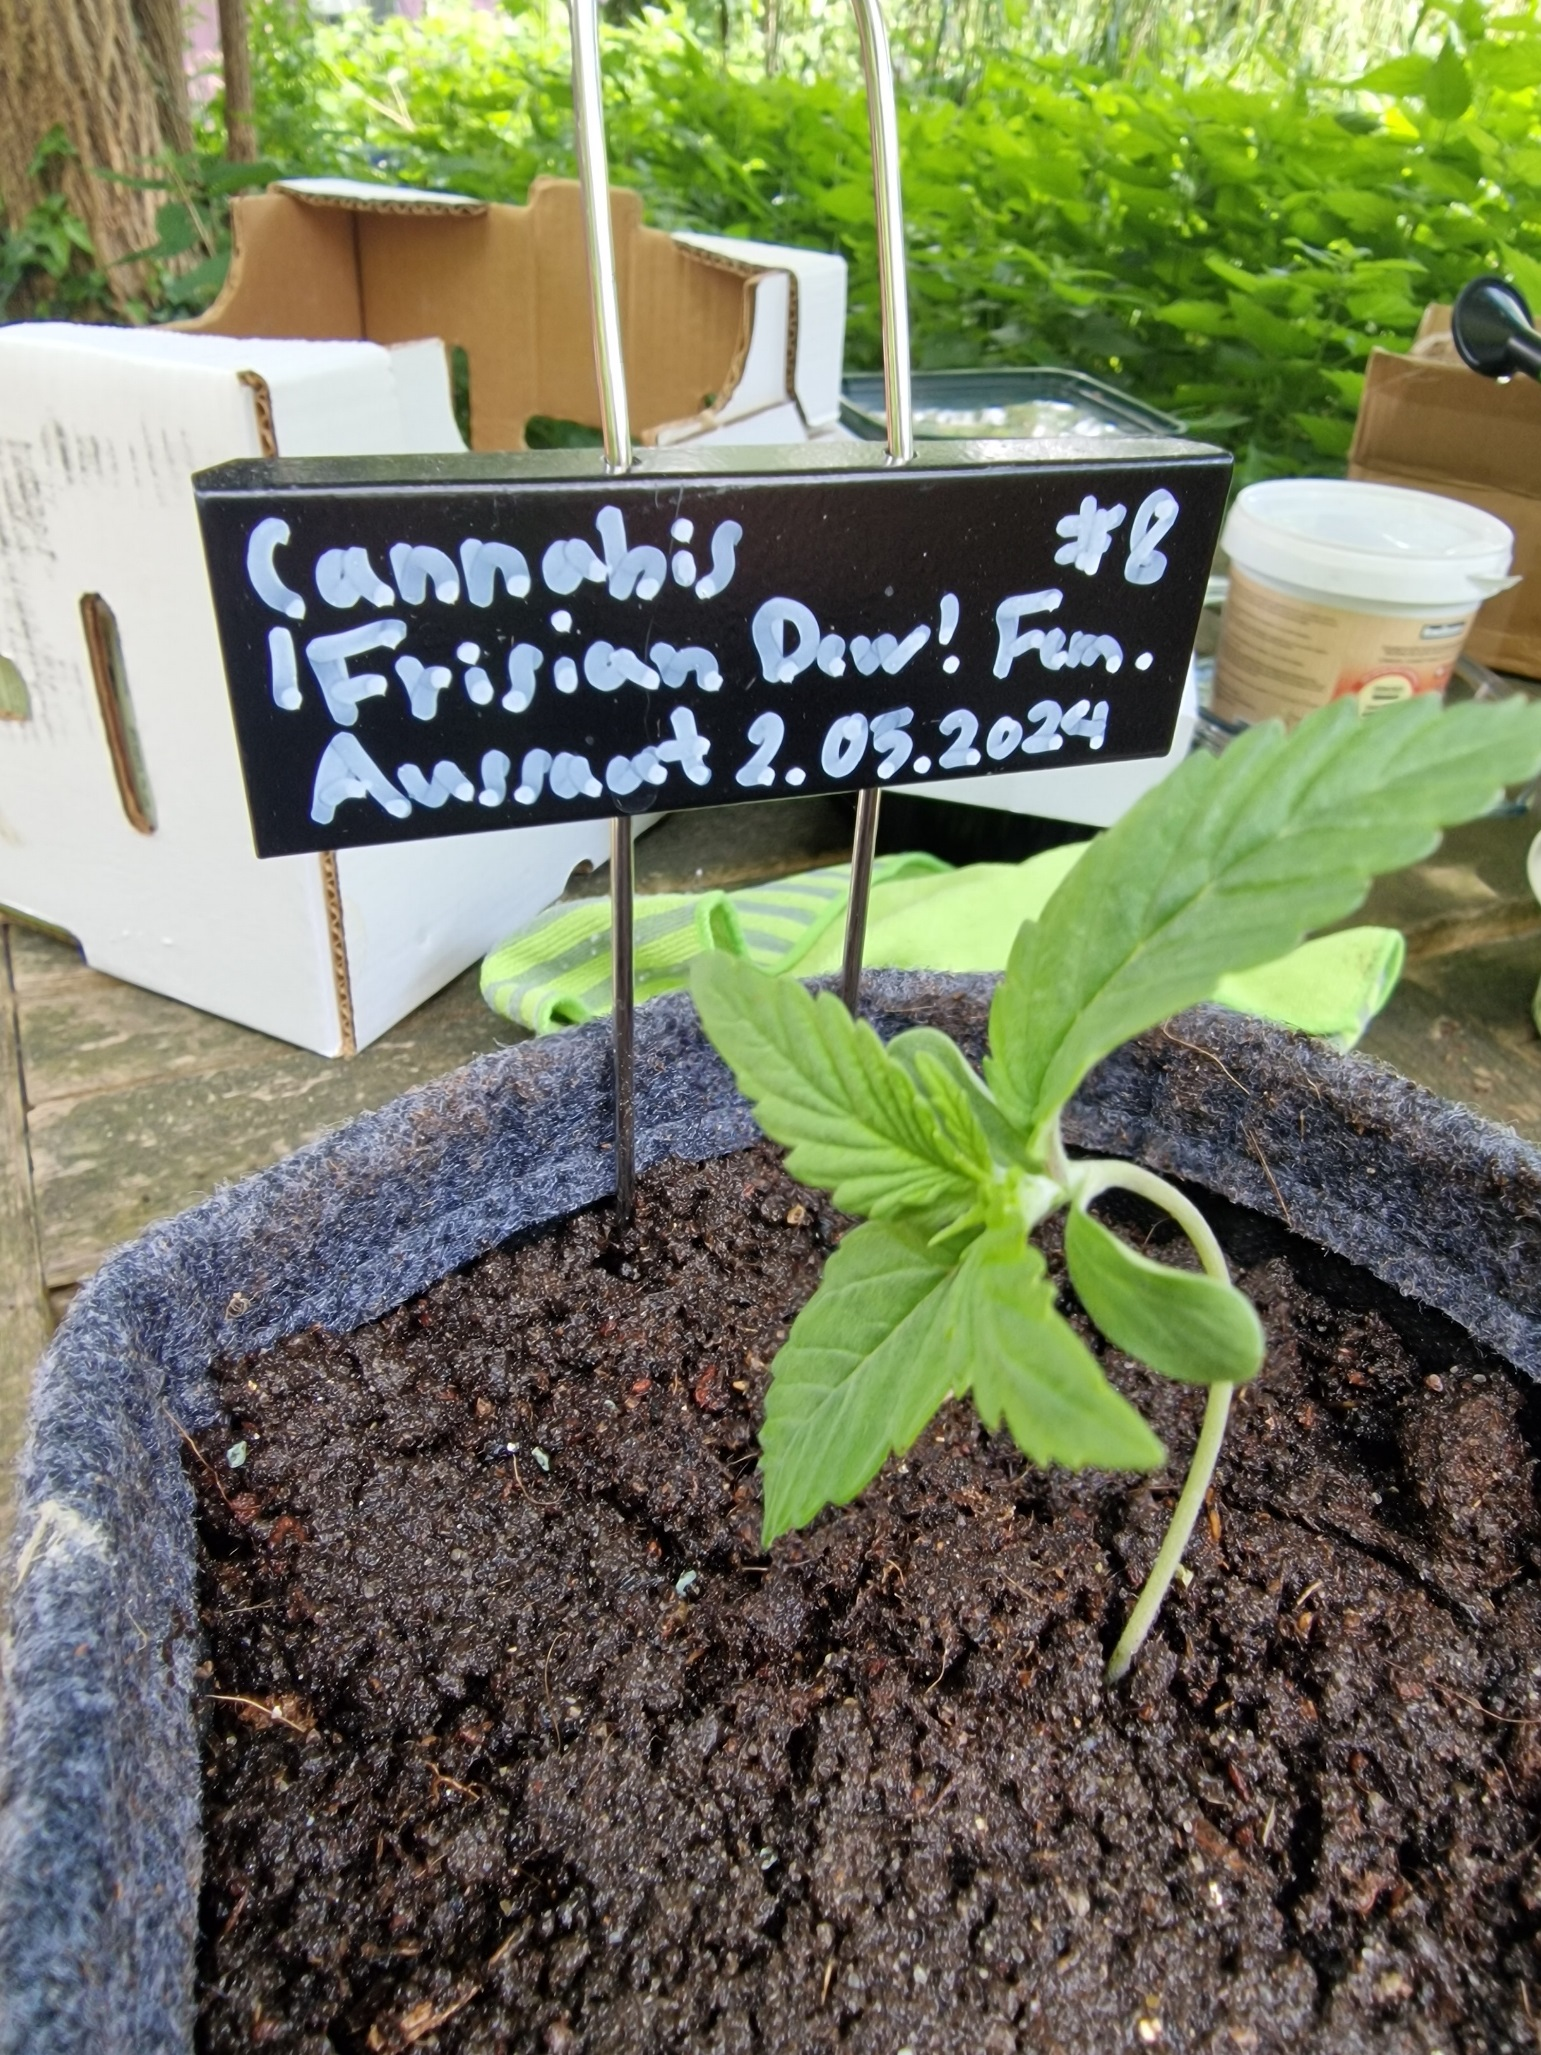
\includegraphics[width=\linewidth]{plant_08_2024-05-13}
        \caption{Plant \# 8}
        \label{fig:plant_08_2024-05-13}
    \end{subfigure}
    \begin{subfigure}[t]{.19\textwidth}
        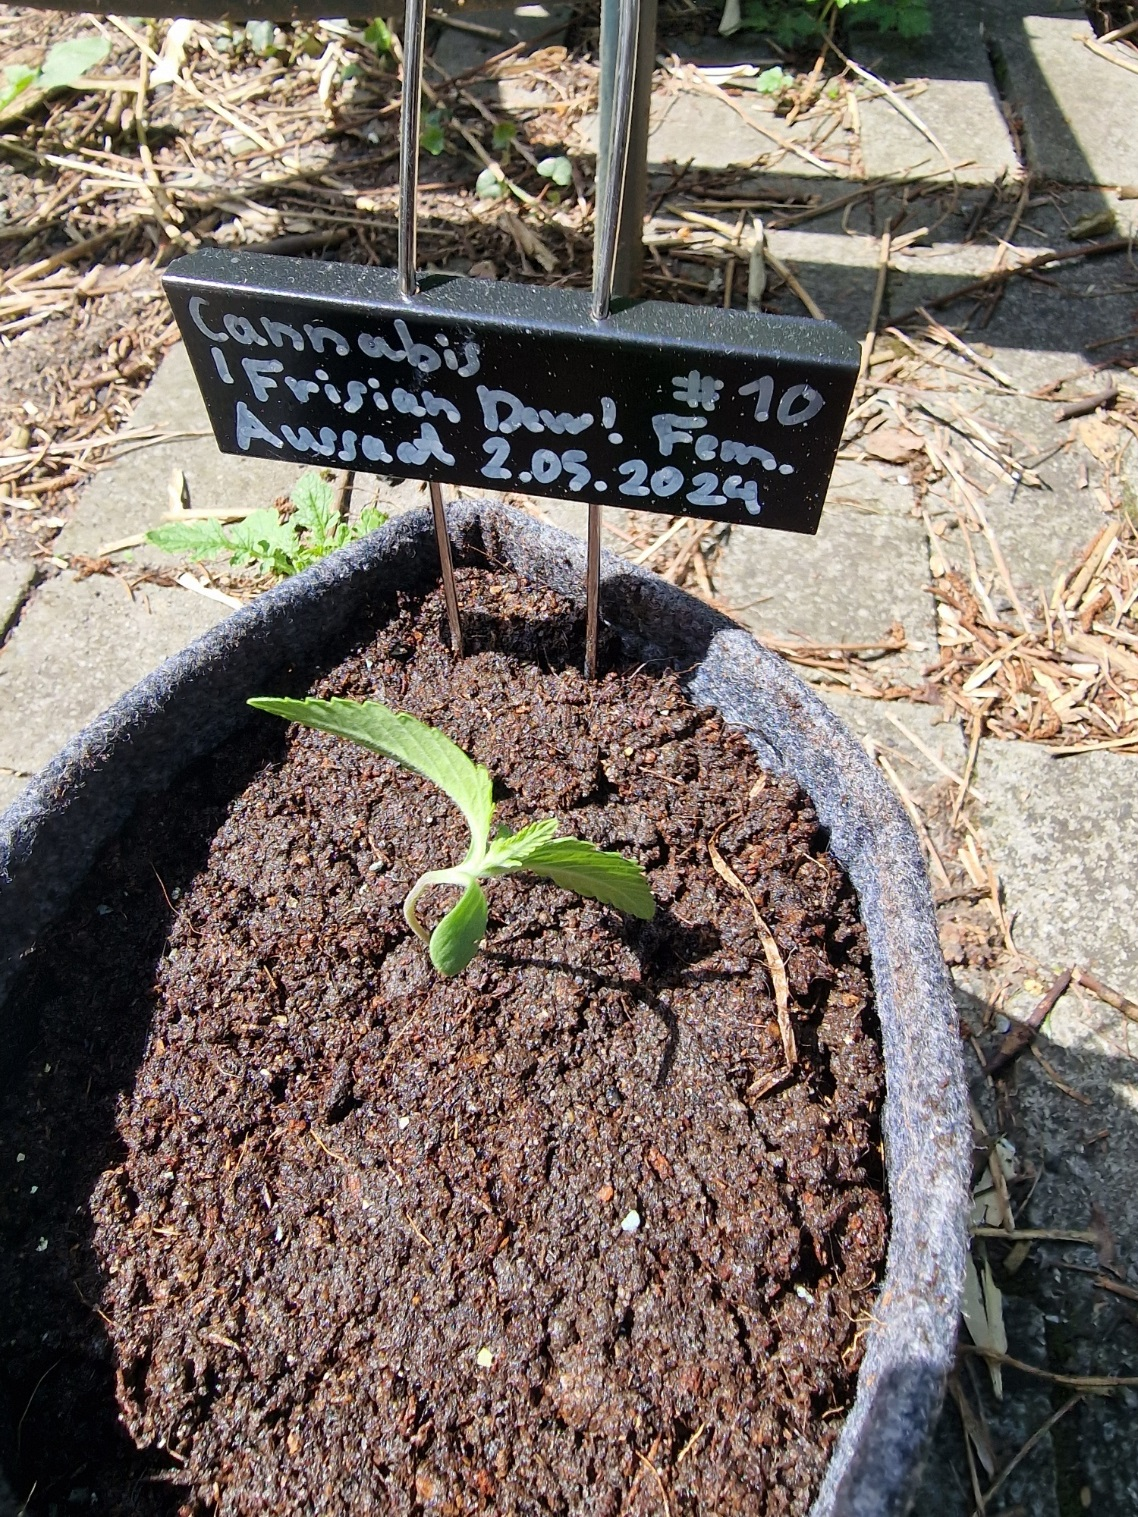
\includegraphics[width=\linewidth]{plant_10_2024-05-13}
        \caption{Plant \# 10}
        \label{fig:plant_10_2024-05-13}
    \end{subfigure}
    \begin{subfigure}[t]{.19\textwidth}
        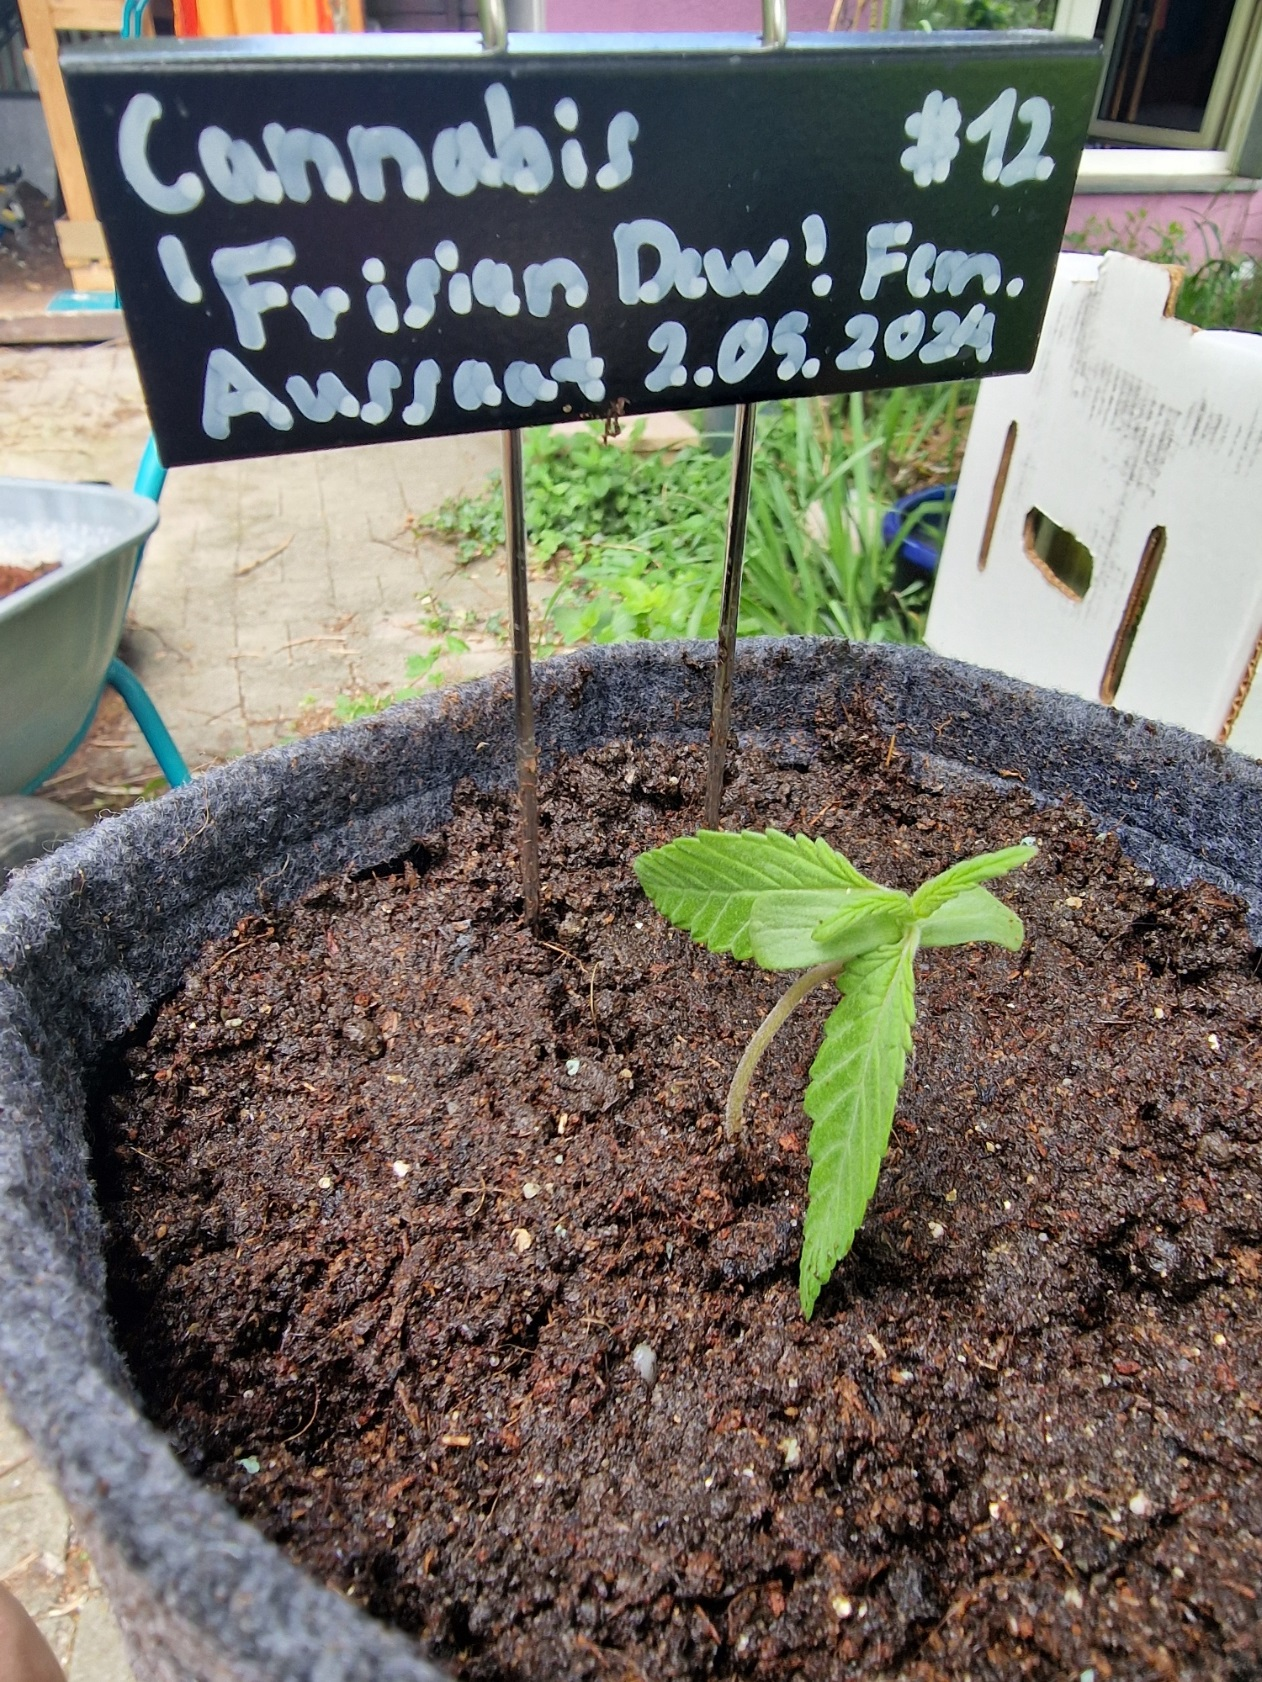
\includegraphics[width=\linewidth]{plant_12_2024-05-13}
        \caption{Plant \# 12}
        \label{fig:plant_12_2024-05-13}
    \end{subfigure}
    \caption[Plants of the control group on May 13]{The plants of the control group on May 13}
    \label{fig:plants_ctrl_2024-05-13}
\end{figure}

\begin{figure}[htbp]
    \begin{subfigure}[t]{.28\textwidth}
        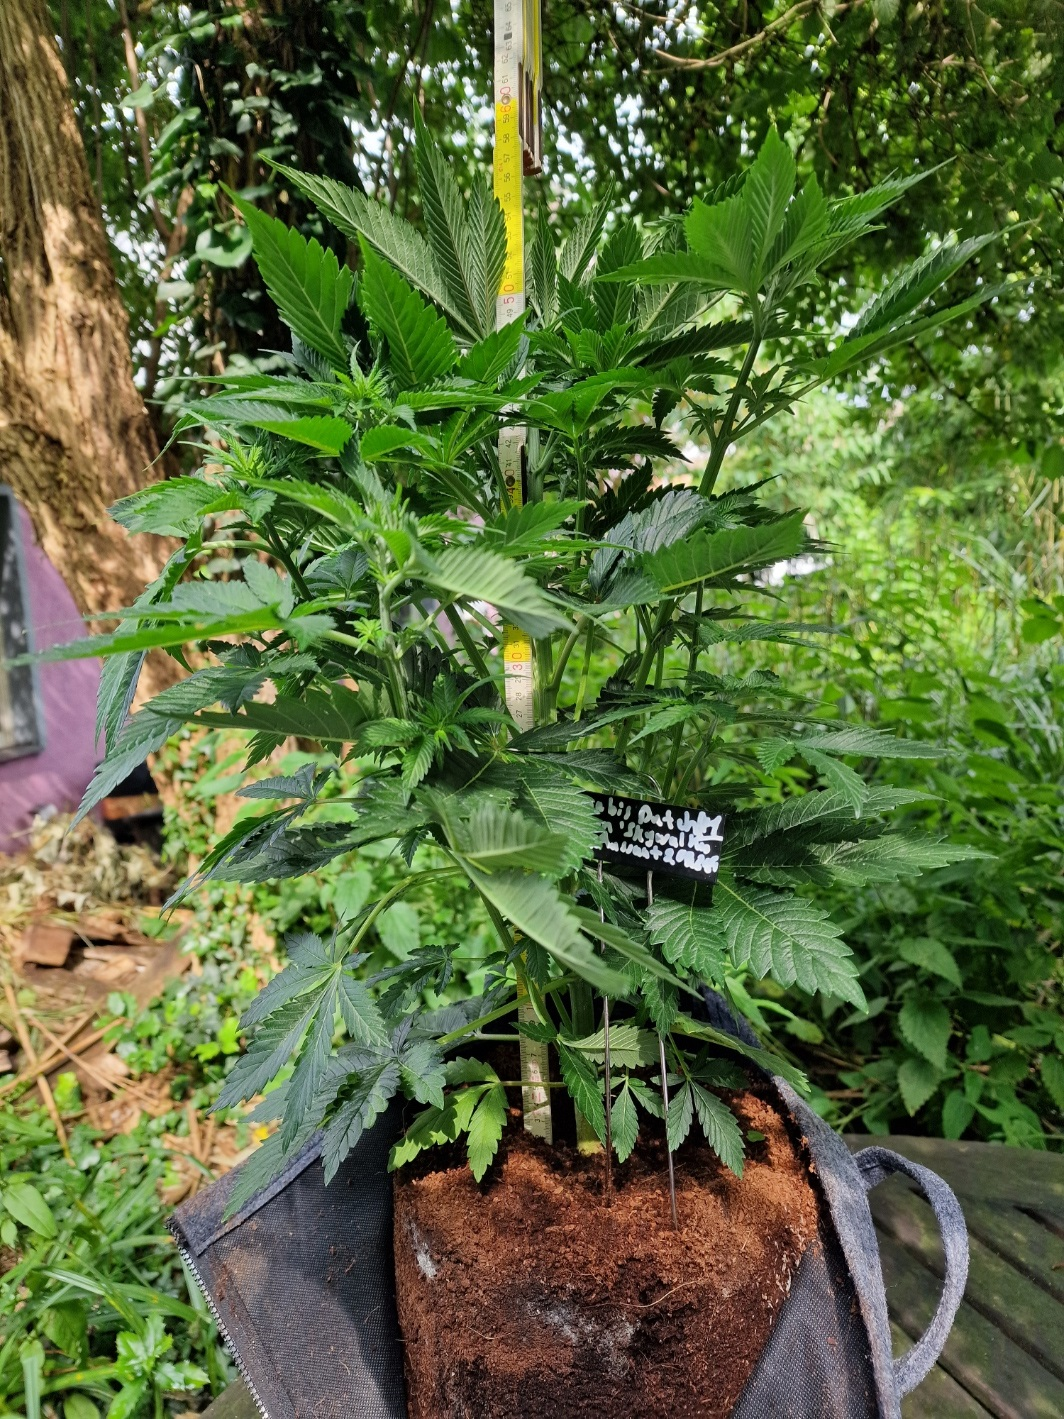
\includegraphics[width=\linewidth]{plant_01_2024-06-17}
        \caption{Plant \# 1}
        \label{fig:plant_01_2024-06-17}
    \end{subfigure}
    \begin{subfigure}[t]{.28\textwidth}
        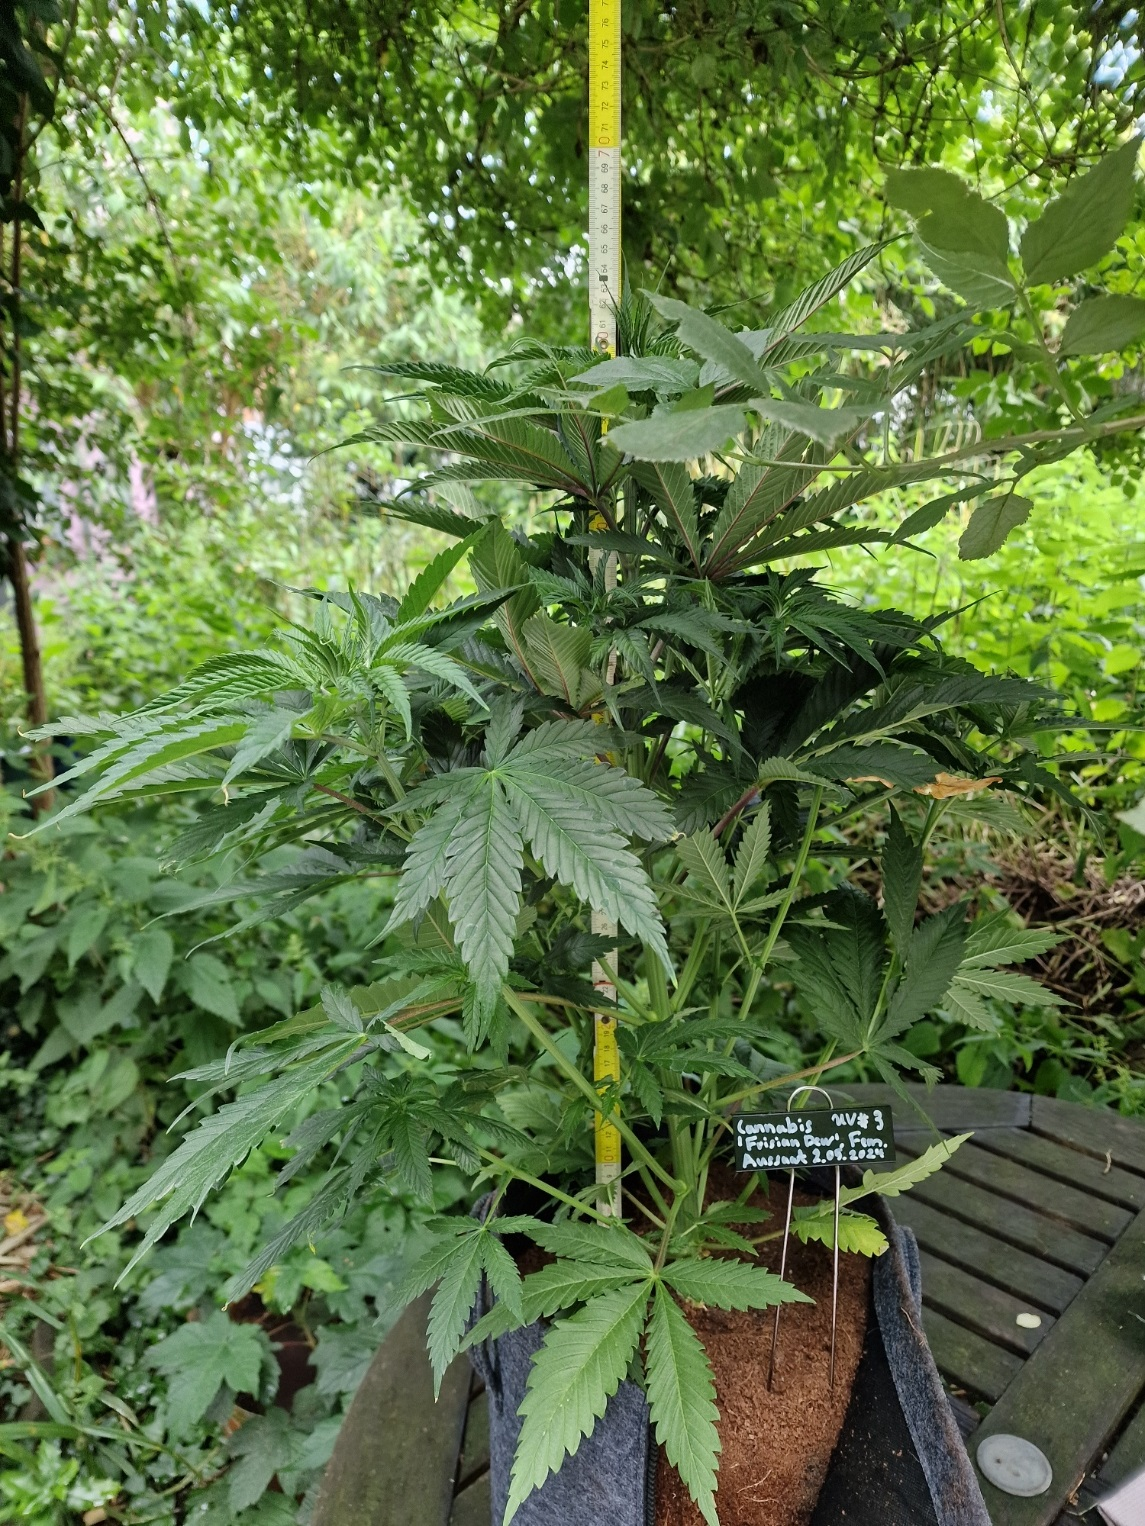
\includegraphics[width=\linewidth]{plant_03_2024-06-17}
        \caption{Plant \# 3}
        \label{fig:plant_03_2024-06-17}
    \end{subfigure}
    \begin{subfigure}[t]{.28\textwidth}
        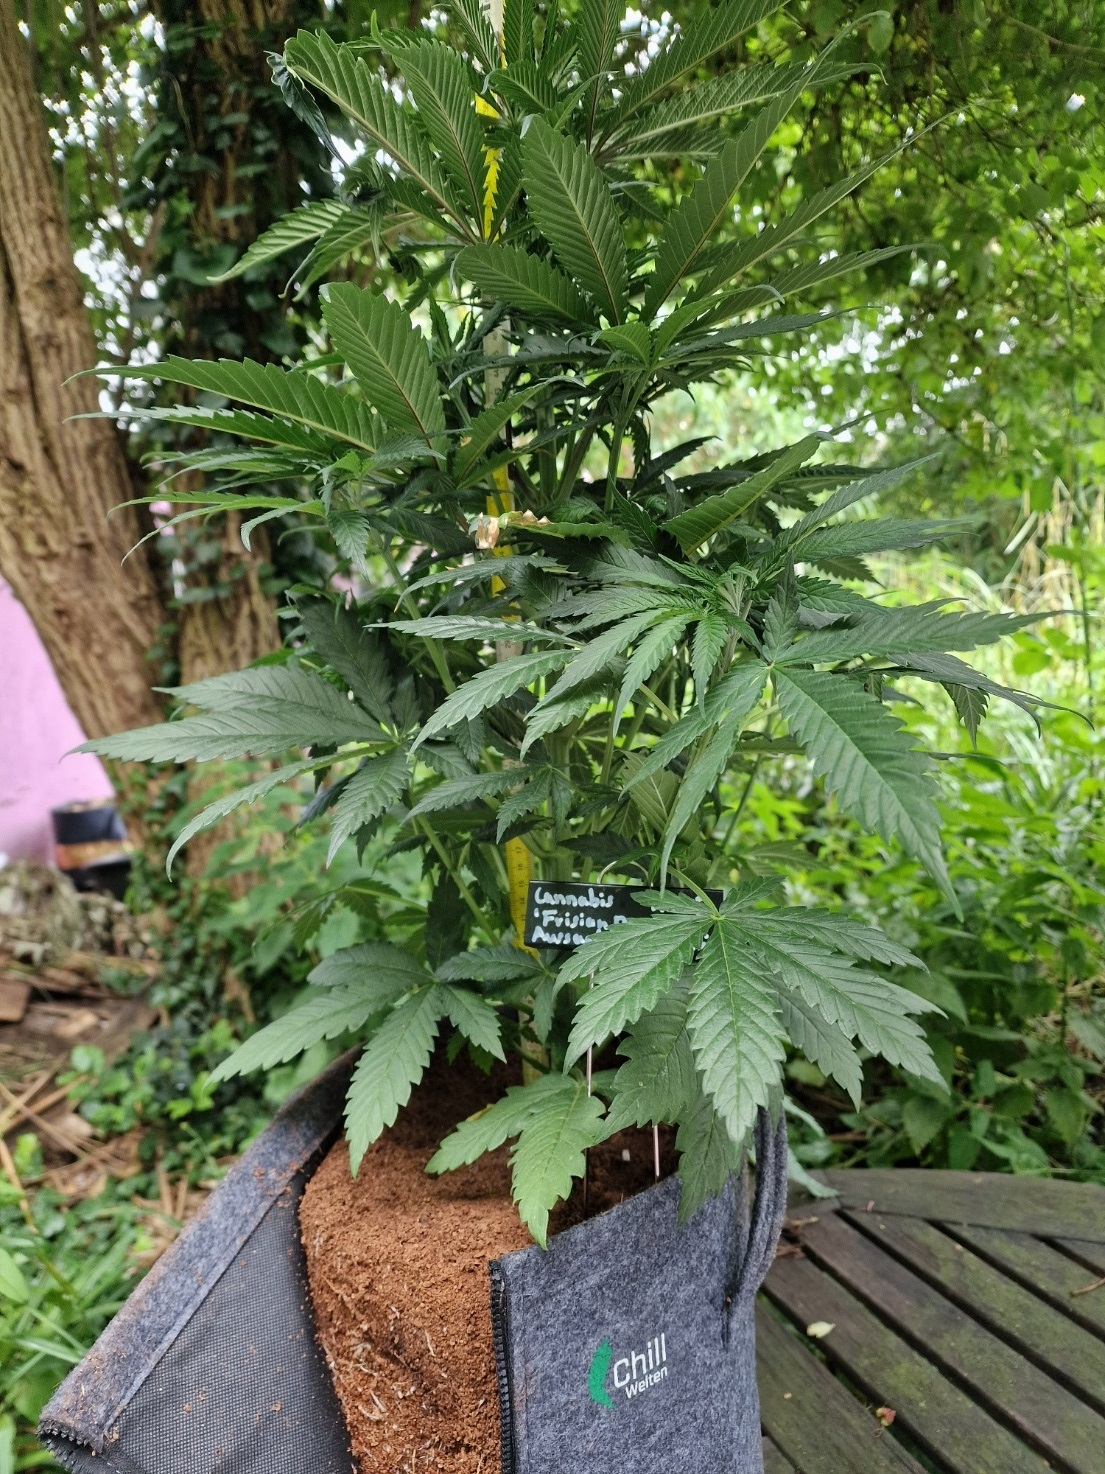
\includegraphics[width=\linewidth]{plant_05_2024-06-17}
        \caption{Plant \# 5}
        \label{fig:plant_05_2024-06-17}
    \end{subfigure}
    \begin{subfigure}[t]{.28\textwidth}
        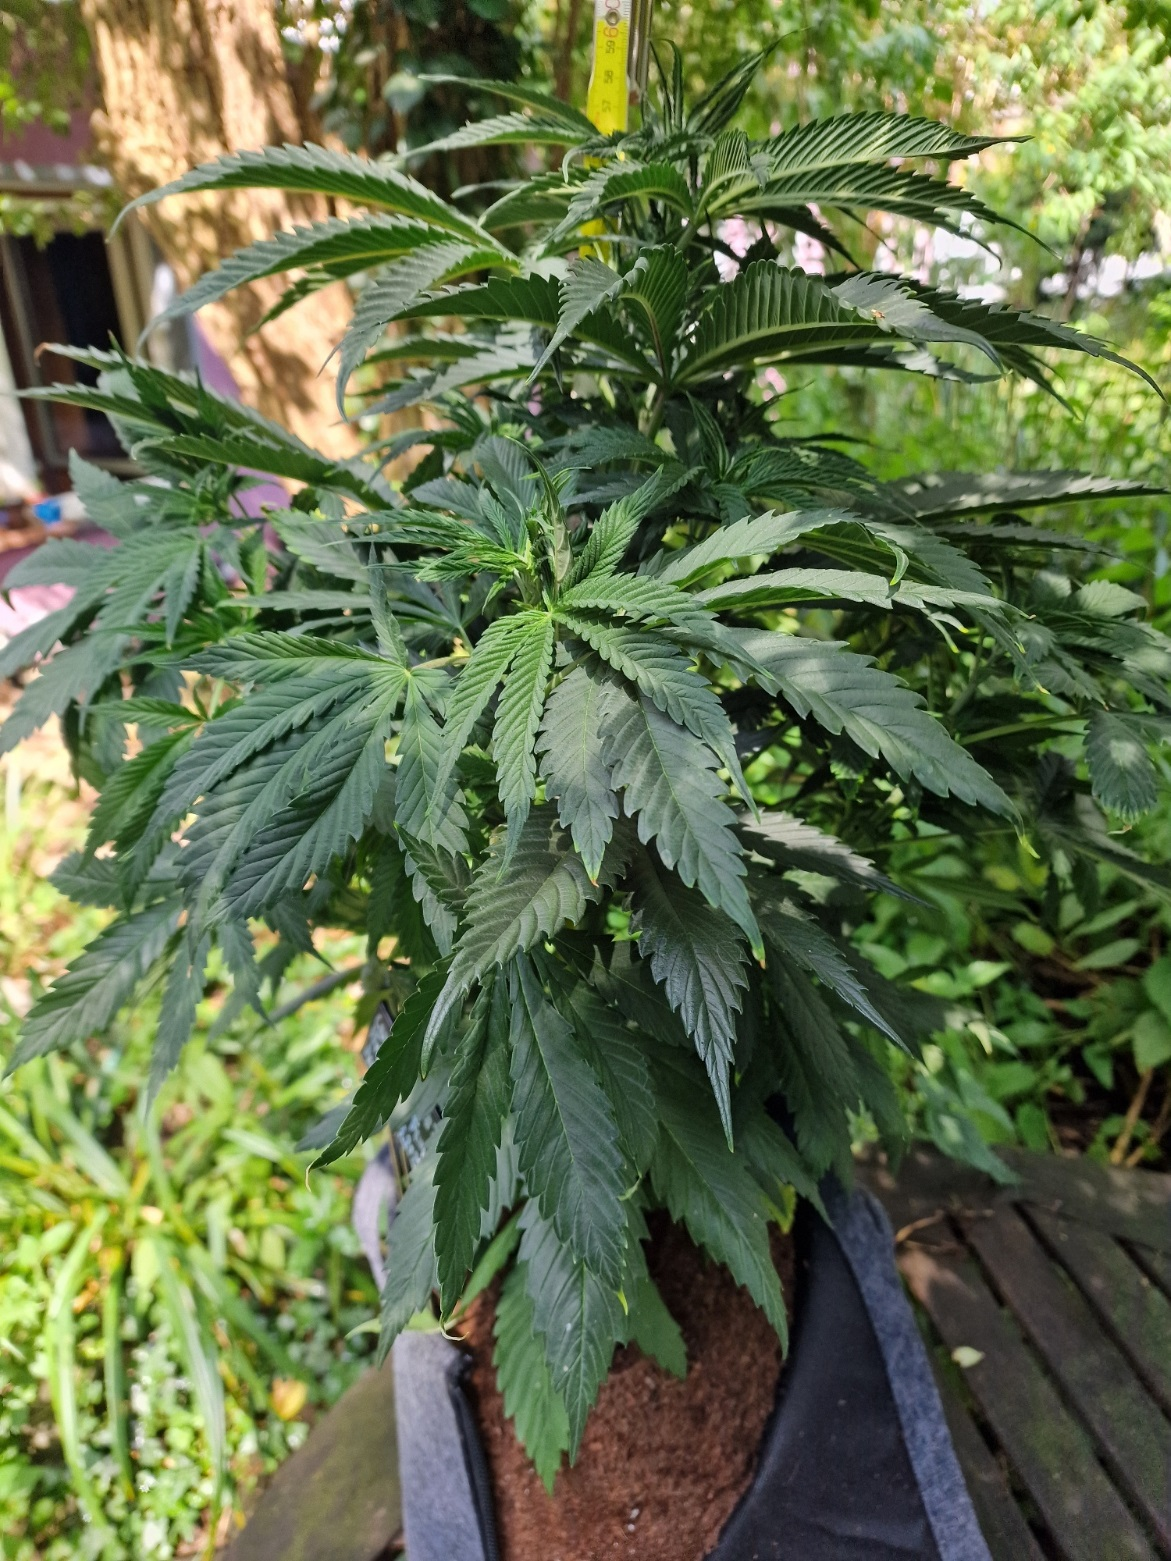
\includegraphics[width=\linewidth]{plant_07_2024-06-17}
        \caption{Plant \# 7}
        \label{fig:plant_07_2024-06-17}
    \end{subfigure}
    \begin{subfigure}[t]{.28\textwidth}
        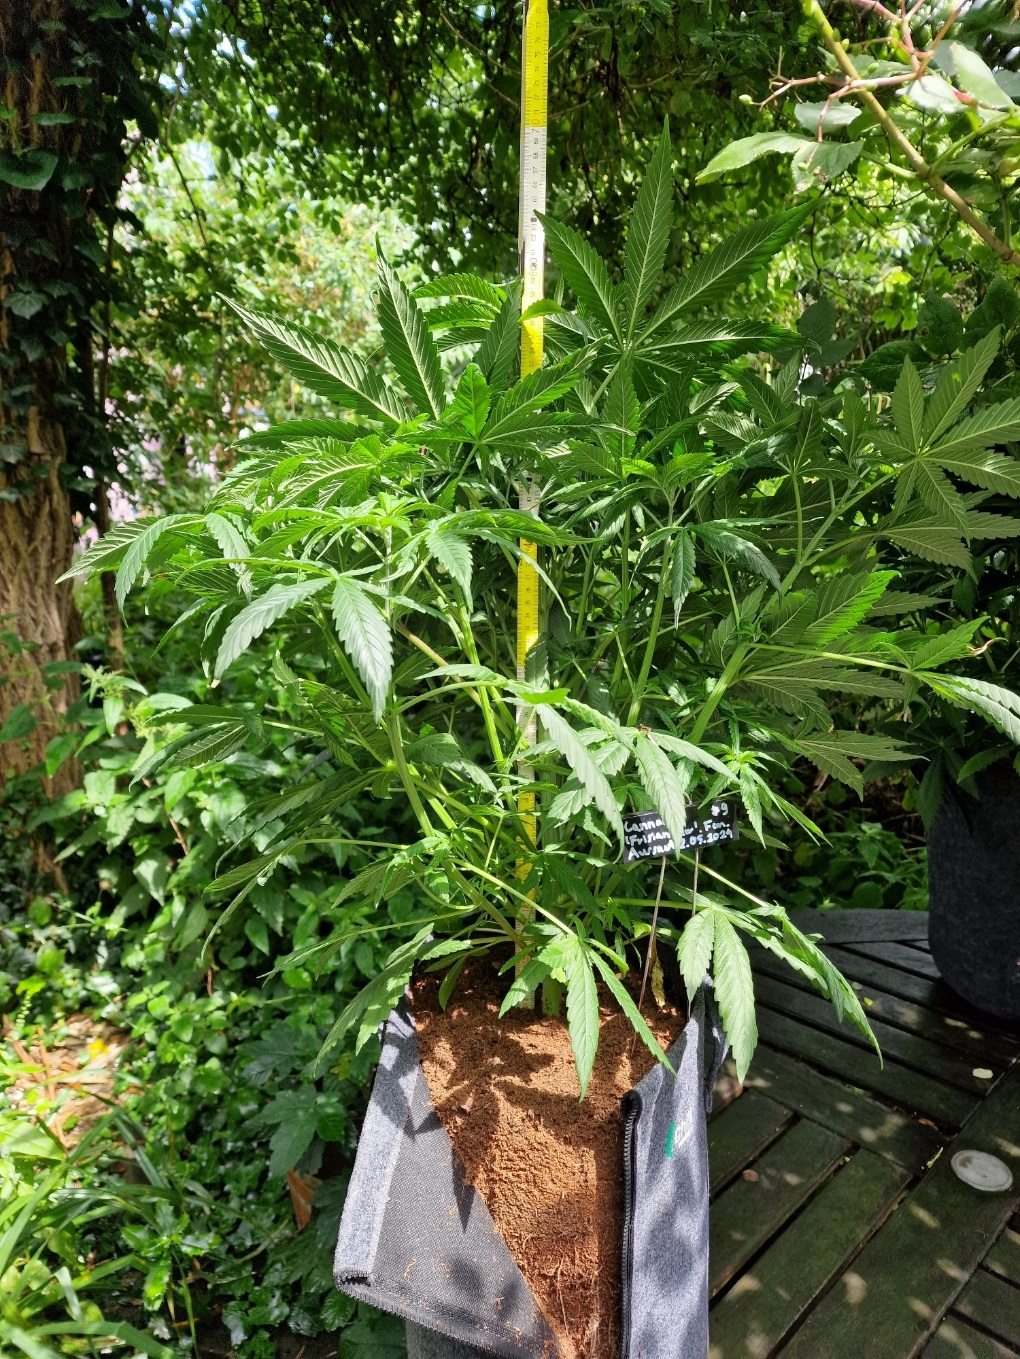
\includegraphics[width=\linewidth]{plant_09_2024-06-17}
        \caption{Plant \# 9}
        \label{fig:plant_09_2024-06-17}
    \end{subfigure}
    \begin{subfigure}[t]{.28\textwidth}
        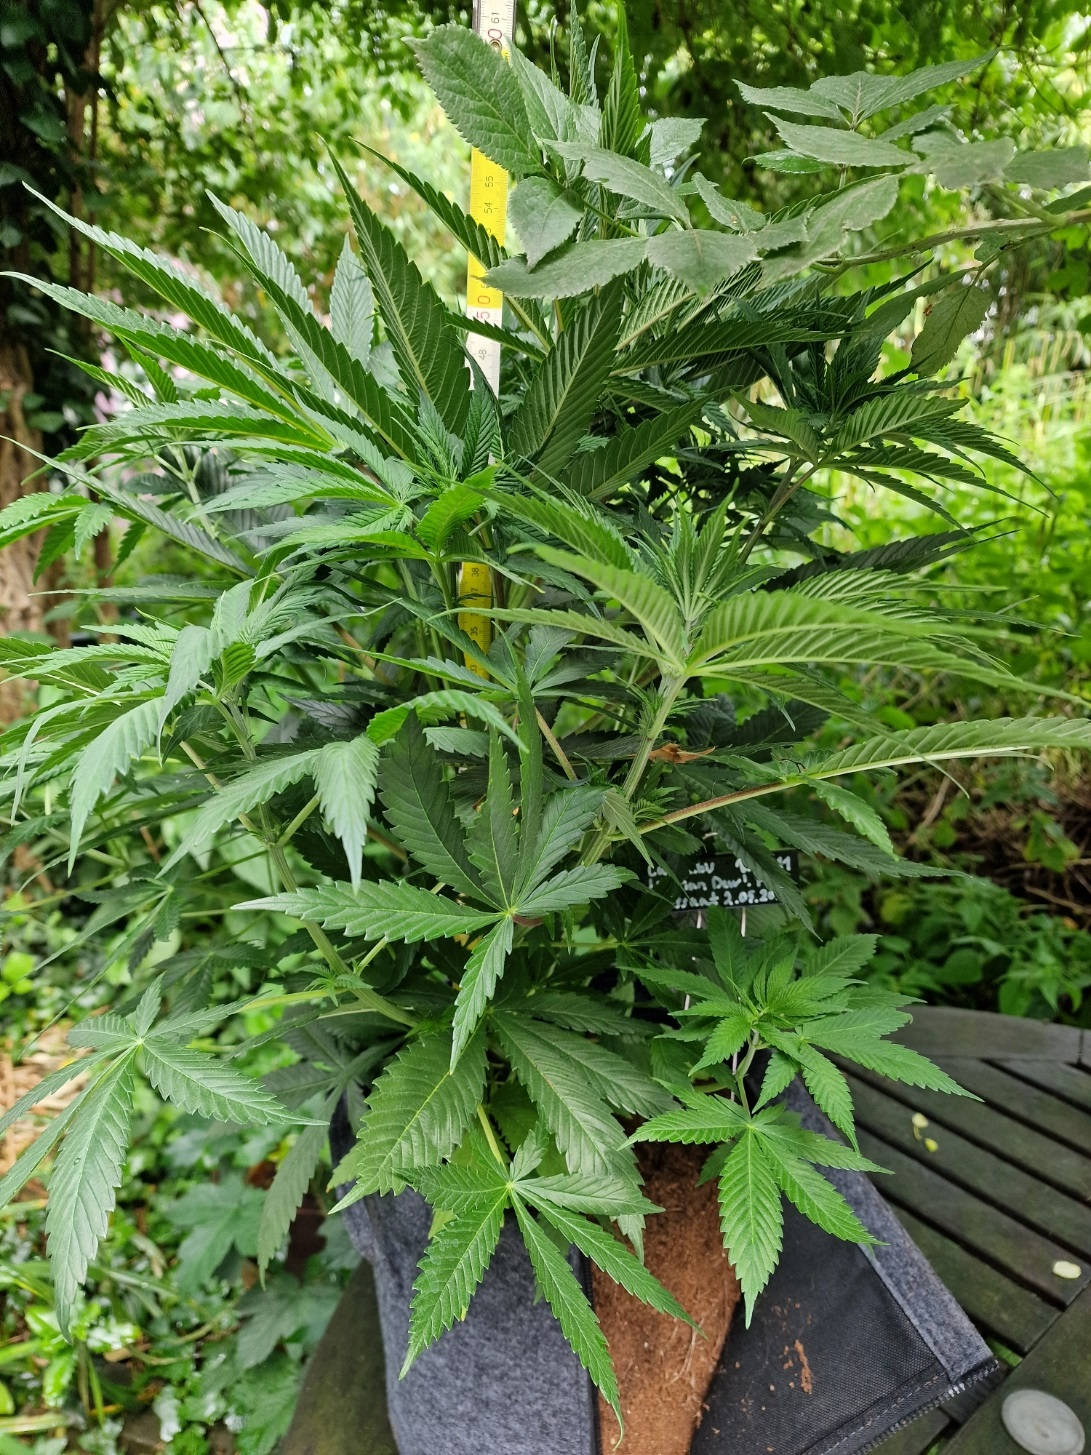
\includegraphics[width=\linewidth]{plant_11_2024-06-17}
        \caption{Plant \# 11}
        \label{fig:plant_11_2024-06-17}
    \end{subfigure}
    \begin{subfigure}[t]{.85\textwidth}
        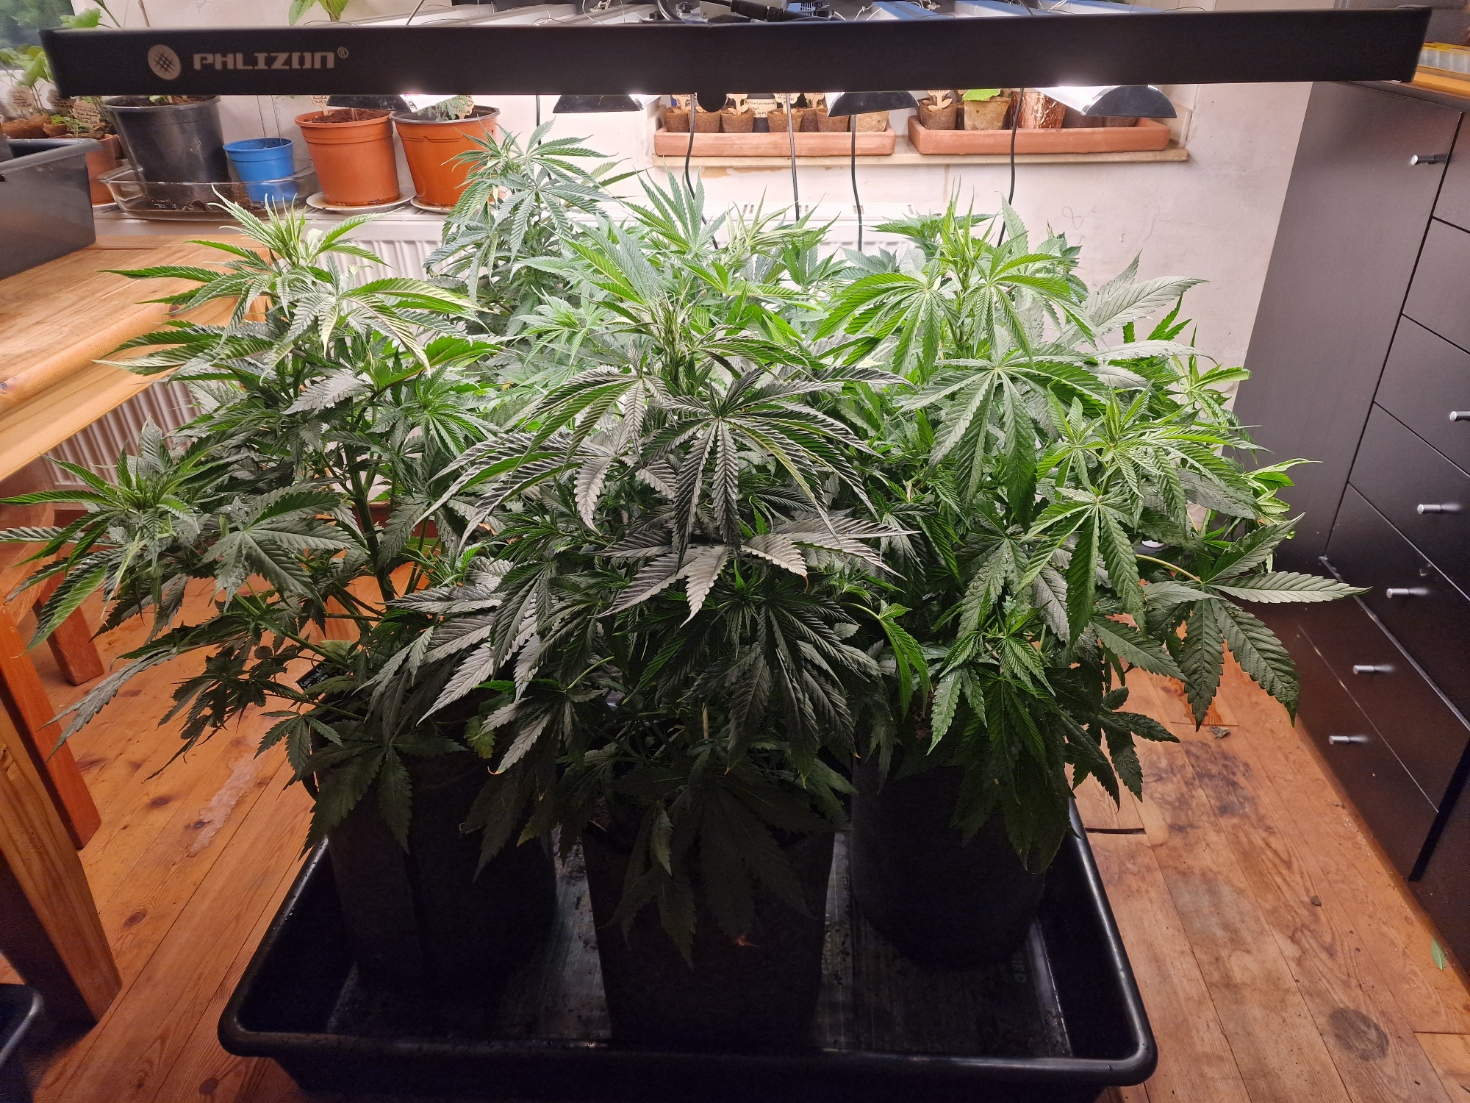
\includegraphics[width=\linewidth]{plant_uv_2024-06-17}
        \caption{All plants of the UV group in their experimental setup under the LED and UV grow lights}
        \label{fig:plant_uv_2024-06-17}
    \end{subfigure}
    \caption[Plants of the UV group on June 17]{The plants treated with UV light on June 17}
    \label{fig:plants_uv_2024-06-17}
\end{figure}

\begin{figure}[htbp]
    \begin{subfigure}[t]{.28\textwidth}
        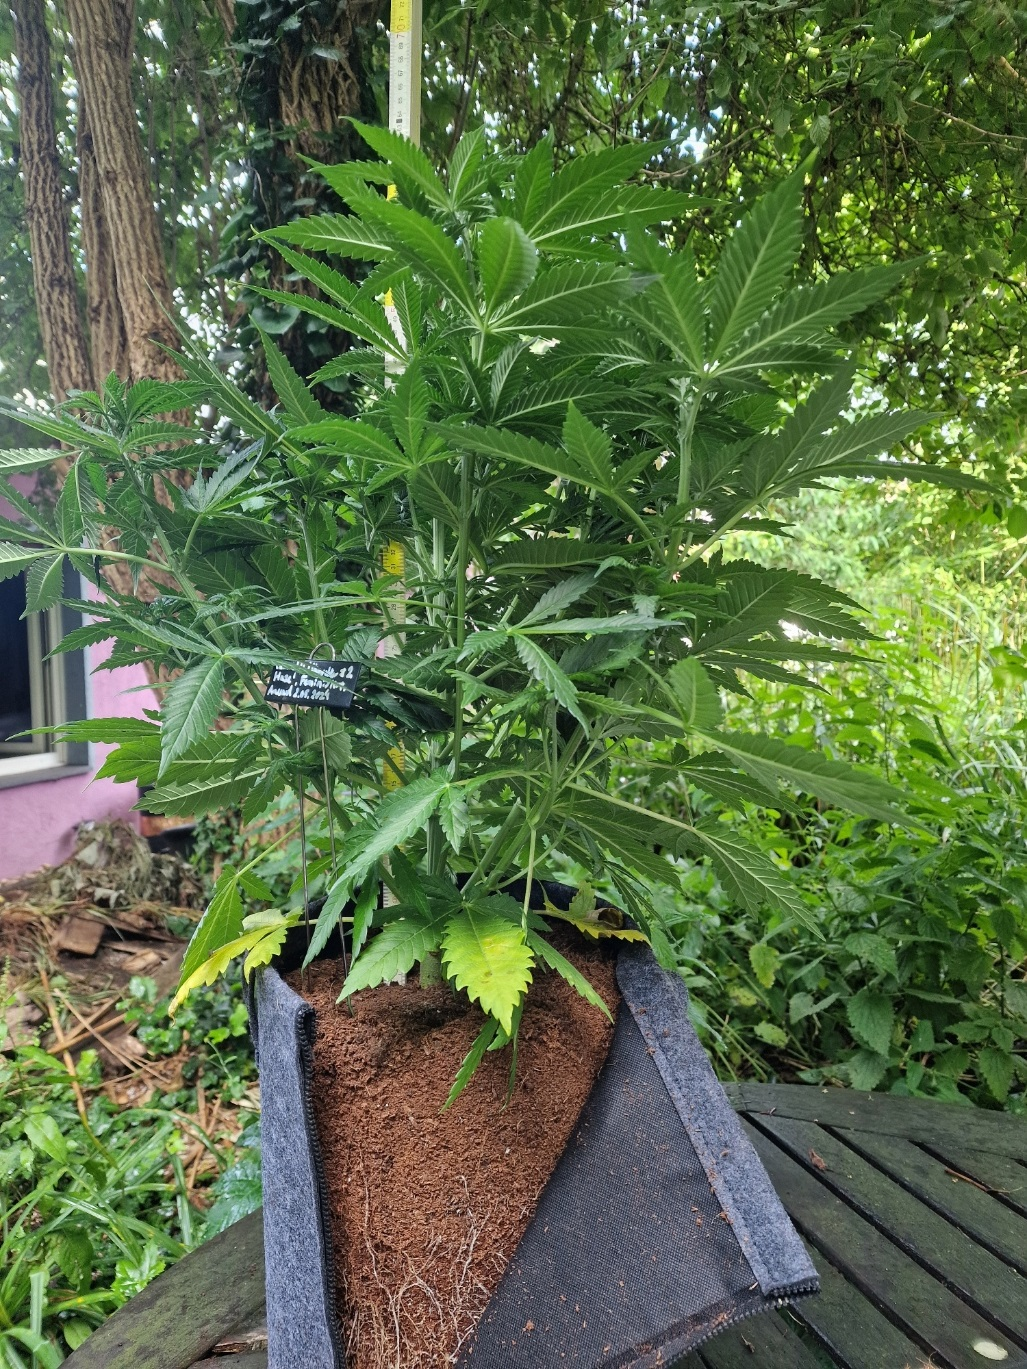
\includegraphics[width=\linewidth]{plant_02_2024-06-17}
        \caption{Plant \# 2}
        \label{fig:plant_02_2024-06-17}
    \end{subfigure}
    \begin{subfigure}[t]{.28\textwidth}
        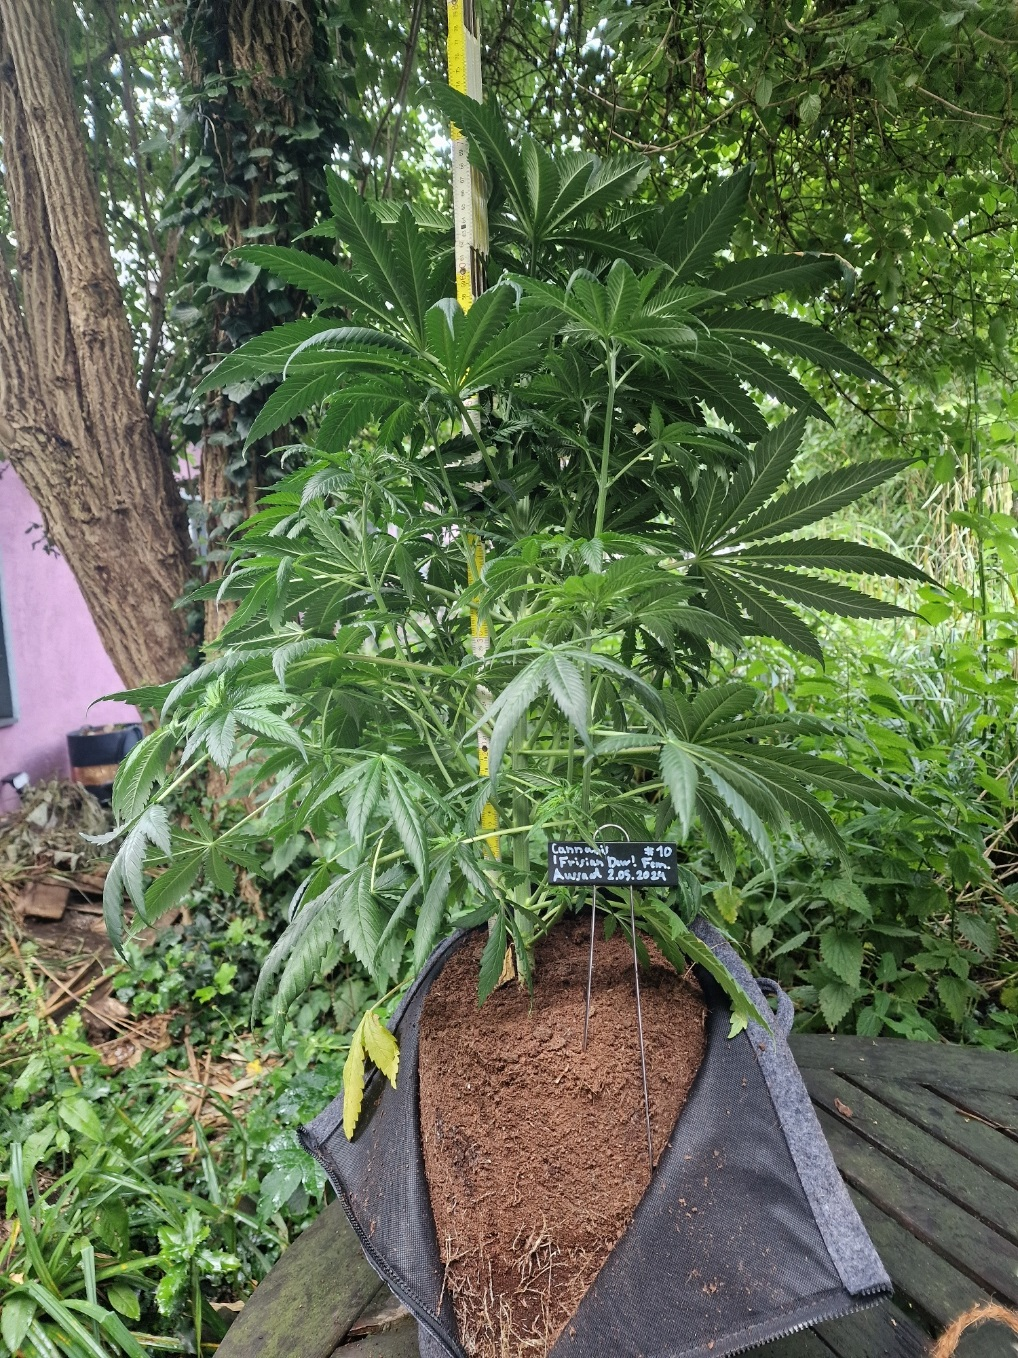
\includegraphics[width=\linewidth]{plant_06_2024-06-17}
        \caption{Plant \# 6}
        \label{fig:plant_06_2024-06-17}
    \end{subfigure}
    \begin{subfigure}[t]{.28\textwidth}
        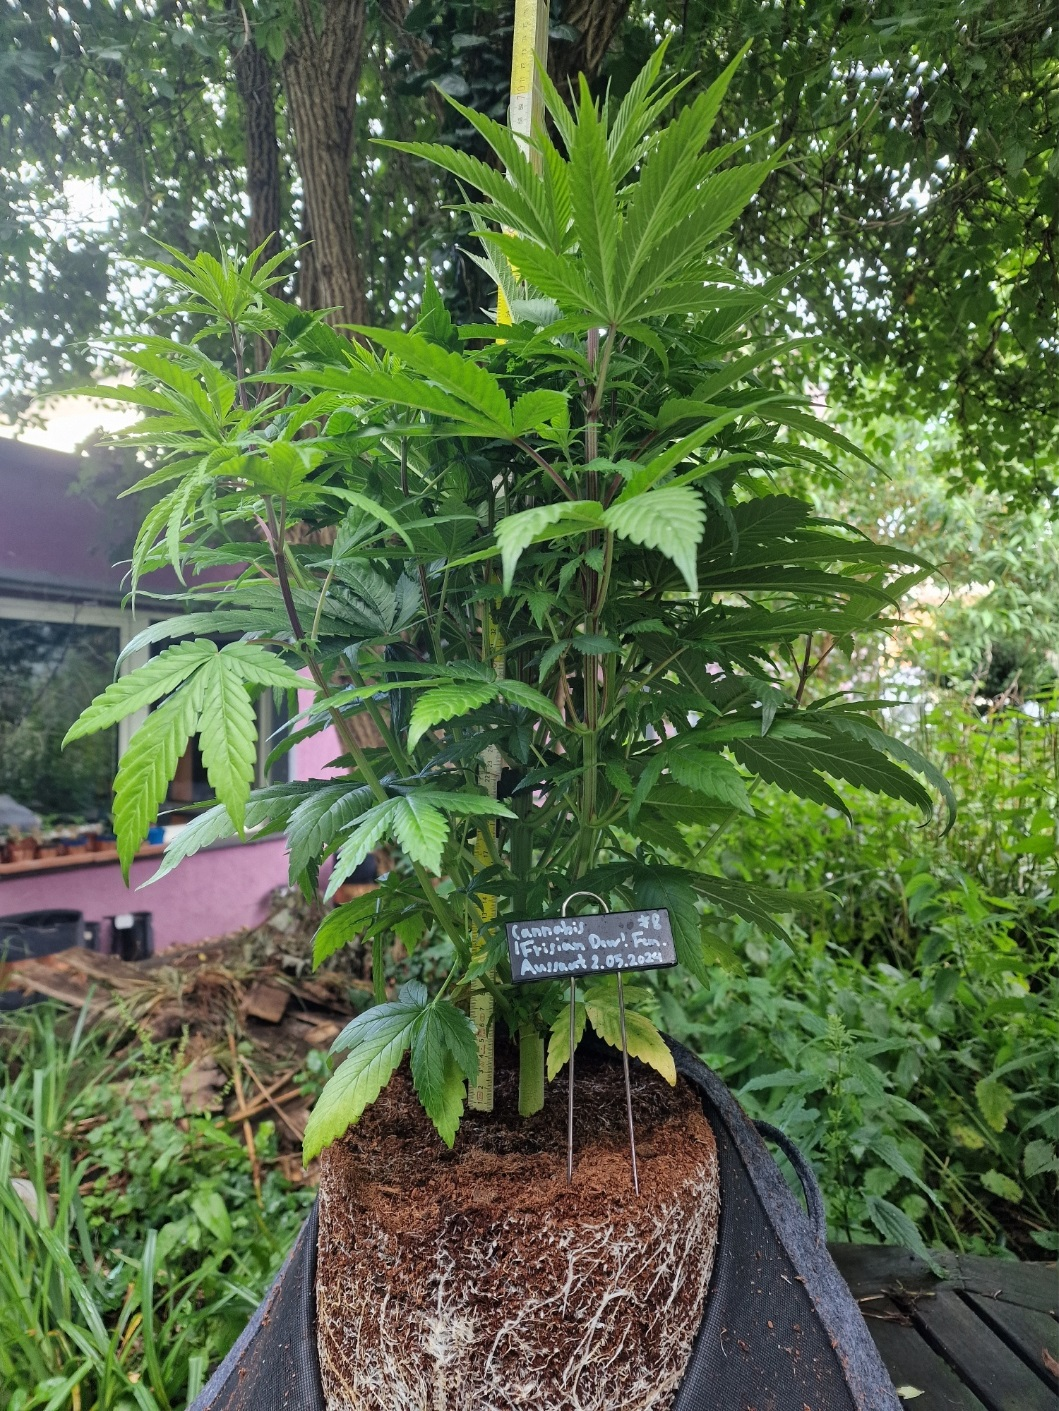
\includegraphics[width=\linewidth]{plant_08_2024-06-17}
        \caption{Plant \# 8}
        \label{fig:plant_08_2024-06-17}
    \end{subfigure}
    \begin{subfigure}[t]{.28\textwidth}
        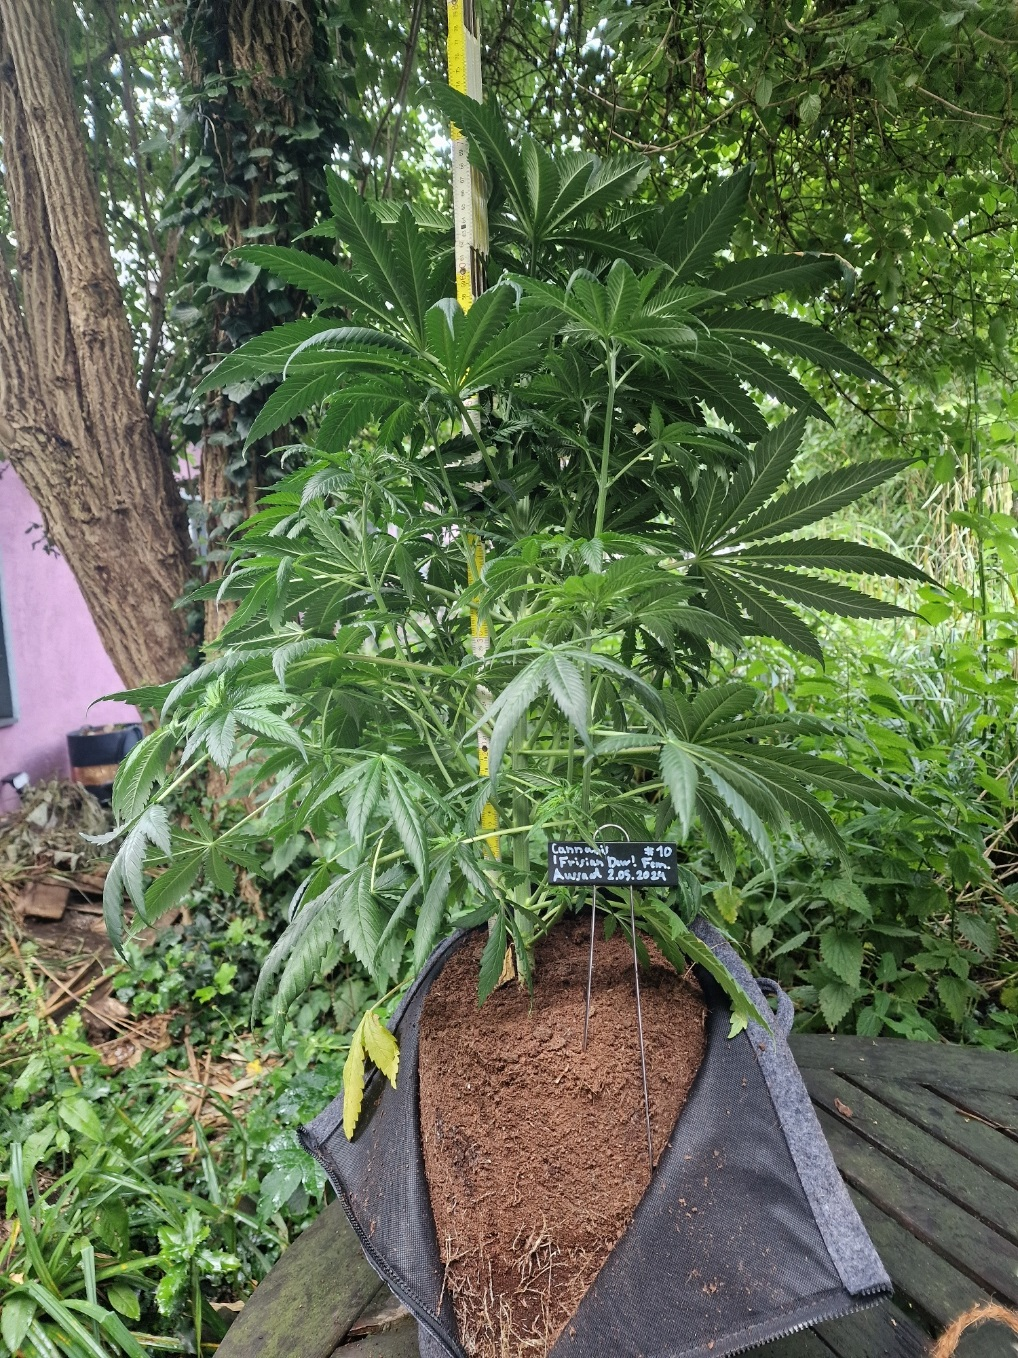
\includegraphics[width=\linewidth]{plant_10_2024-06-17}
        \caption{Plant \# 10}
        \label{fig:plant_10_2024-06-17}
    \end{subfigure}
    \begin{subfigure}[t]{.28\textwidth}
        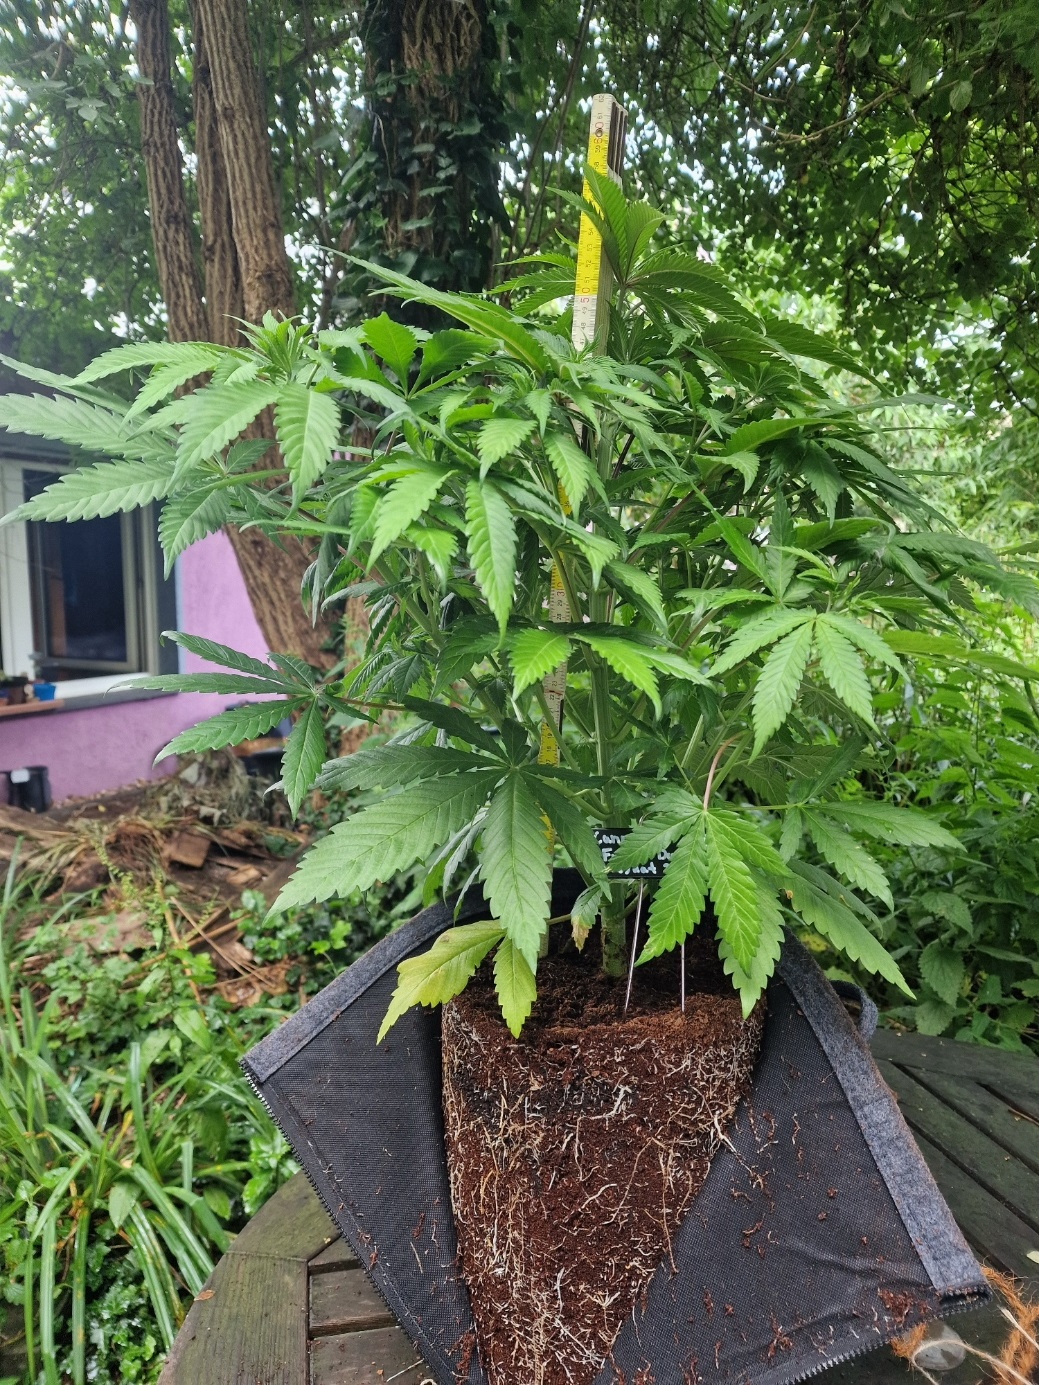
\includegraphics[width=\linewidth]{plant_12_2024-06-17}
        \caption{Plant \# 12}
        \label{fig:plant_12_2024-06-17}
    \end{subfigure}
    \begin{subfigure}[t]{.85\textwidth}
        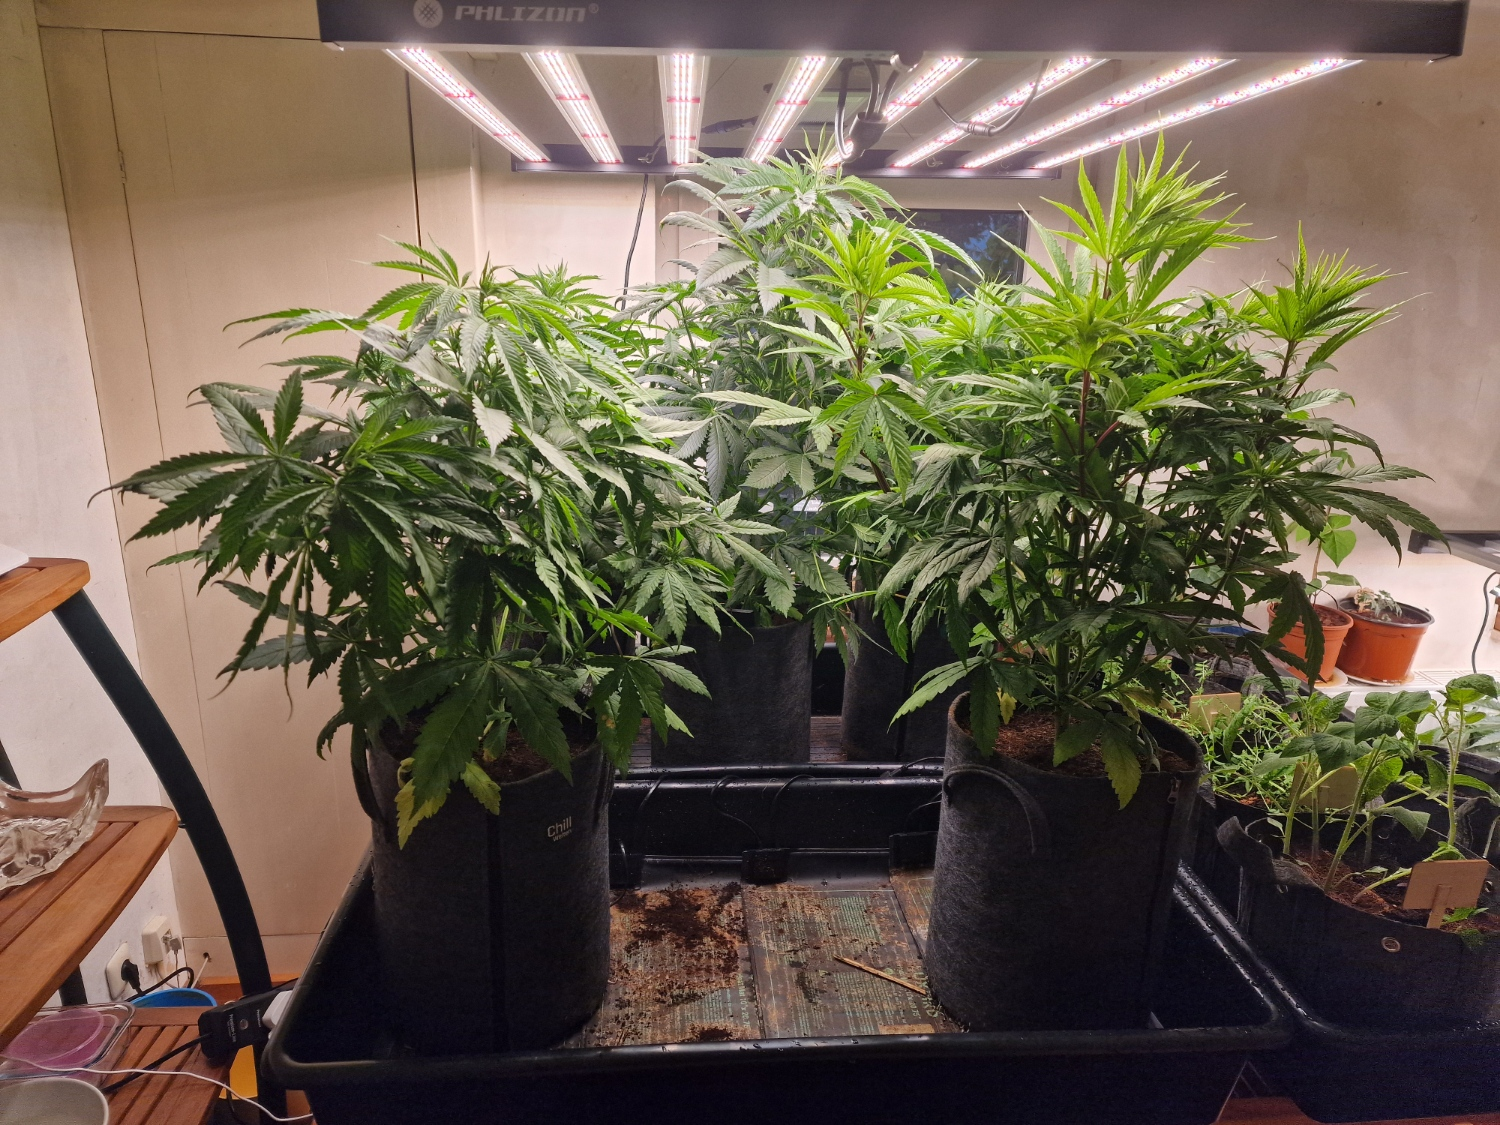
\includegraphics[width=\linewidth]{plant_ctrl_2024-06-17}
        \caption{All plants of the control group in their experimental setup under the LED grow lights}
        \label{fig:plant_ctrl_2024-06-17}
    \end{subfigure}
    \caption[Plants of the control group on June 17]{The plants of the control group on June 17}
    \label{fig:plants_ctrl_2024-06-17}
\end{figure}

\begin{figure}[htbp]
    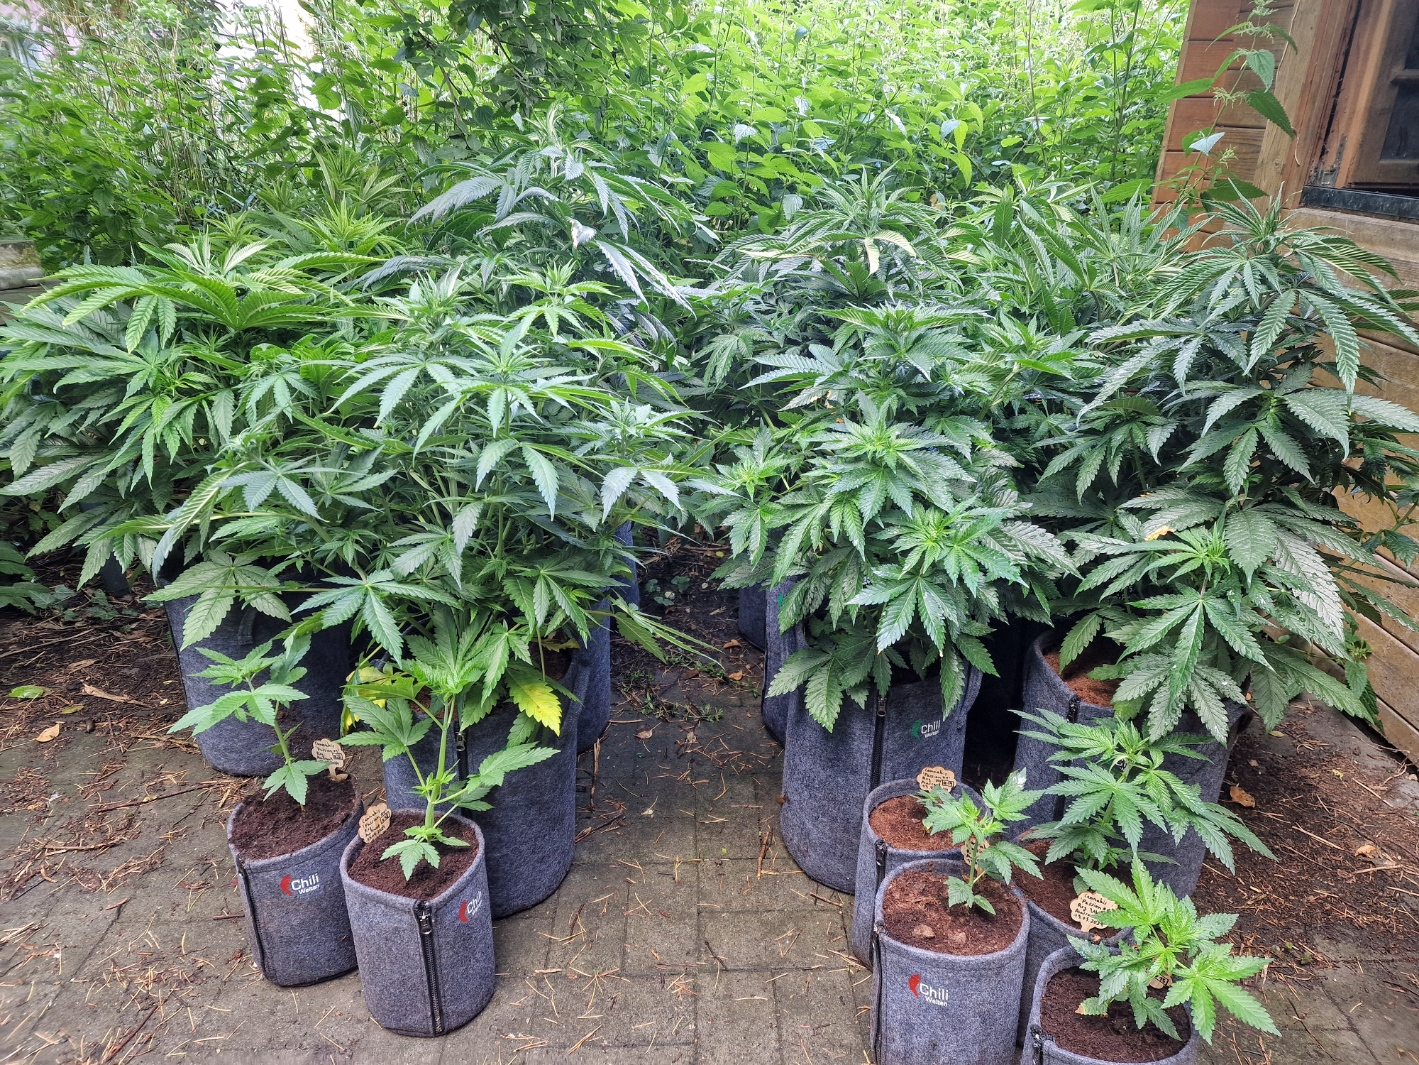
\includegraphics[width=\linewidth]{plant_all_2024-06-17}
    \caption[Plants of both the UV and control groups on June 17]{All plants of both the UV and control groups on June 17. The control group plants are arranged on the left, while the UV group plants are on the right.}
    \label{fig:plant_all_2024-06-17}
\end{figure}

    \newpage
    \section{Discussion}

The initial hypothesis of this experiment was that exposure to UV light at controlled low intensities would enhance the germination rate and seedling development of cannabis seeds by inducing protective and growth-promoting biochemical responses. However, the results of this study indicate no significant differences in plant height, stem circumference, or number of internodes between the UV and control groups for the Frisian Dew cultivar.

These findings suggest that the controlled low-intensity UV exposure used in this experiment did not significantly influence the measured growth parameters under the given conditions. This could be due to several factors, including the possibility that the UV exposure level was insufficient to induce noticeable changes in growth parameters.

While the primary focus of this experiment was on growth parameters, it is important to consider other potential benefits of UV exposure that were not directly measured in this study. For example, UV light has been shown to increase the production of secondary metabolites such as cannabinoids and flavonoids, which are important for the plant's defense mechanisms and have significant pharmacological properties. Enhanced production of these compounds could improve the quality and potency of cannabis plants, even if growth parameters remain unchanged.

Additionally, acclimating cannabis seedlings to UV light indoors could have practical benefits for outdoor cultivation. Plants accustomed to UV exposure might be better prepared to handle natural sunlight, potentially leading to improved growth and resilience when transplanted outdoors.

Future experiments could explore these aspects in more detail by including measurements of cannabinoid\index{metabolite!cannabinoid} and flavonoid\index{metabolite!flavonoid} content, as well as examining longer exposure durations and varying intensities of UV light. Moreover, it would be beneficial to study the combined effects of UV light with other environmental factors, such as temperature and humidity, to develop a more comprehensive understanding of how to optimize indoor cultivation conditions for cannabis.

In summary, while the current study did not find significant differences in growth parameters between the UV and control groups, it highlights the need for further research into the broader effects of UV light on cannabis plants. By expanding the scope of future studies, we can better understand how to leverage UV exposure to enhance both the growth and biochemical profiles of cannabis plants.

    \clearpage

    \printbibliography[heading=bibintoc]

    \clearpage

    \printindex
\end{document}